\chapter{Translation}
\label{ch:translation}

\textbf{This chapter is now complete - but wasn't in the first three chapter draft submission!}

In this chapter, we discuss the translation process from C++ to Rust of the selected mini-app, HPCCG. First, we introduce the implementation details of HPCCG, along with the translation methodology undertaken. Then, we present a sequence of incrementally performant translations, showing how features of and packages for the Rust language can contribute to the performance of translations of C++ codebases. Next, we discuss approaches for checking program equivalence, which is critical to guarantee performance comparisons are fair. Finally, we conclude with a section on lessons learned from the process, and a proposed workflow for engineers translating High-Performance C++ codebases to Rust.

% The overall goal of this effort is to generate a software product -- a Rust translation of the HPCCG codebase, with strong performance running in serial, and whilst leveraging shared and distributed memory parallelism. On top of this, we propose a approaches for equivalence checking such translations, and use them to give confidence the Rust translation of HPCCG can be used for fair performance comparisons with the reference C++ version.

As discussed in \Cref{ch:background}, this translation effort is novel with respect to assessing High-Performance Computing for a number of reasons. Previous literature has translated only single computation kernels \cite{bychkovRustLanguageSupercomputing2021} with support for shared and distributed memory parallelism, or very short ``toy example'' applications of around only 150 lines \cite{costanzoPerformanceVsProgramming2021} \cite{moranEmergingTechnologiesRust2023} with support for only shared memory parallelism.

Contrasting this, HPCCG is a standard mini-app as part of the Mantevo suite, with the C++ version totalling 1524 lines and having support for both shared and distributed memory parallelism. This order of magnitude increase in codebase length over modern existing work and support for distributed memory parallelism outside of single computation kernel contexts is both novel and provides a valuable insight into the suitability of Rust in High-Performance Computing.

\section{Design}
\label{sec:translation-design}

In traditional software development tasks, such as building the HPC MultiBench tool discussed in \Cref{ch:hpc-multibench}, system design is paramount to building a coherent product. However, for translation tasks the reference implementation has already been designed. As a result of this, the majority of the effort is in understanding the codebase to be translated, and identifying difficulties arising from the differences in program model between the original and target language.

\subsection{Differences in the Rust and C++ programming models}
\label{sec:rust-cpp-programming-models}

Every programming language can be though of as presenting a different abstraction over the capabilities of a variety of physical computer hardware. For low-level languages such as x86 Assembly, this abstraction directly maps to the machine code instructions executed on the bare metal. Above this, languages such as C provide abstractions for common structures such as iteration, but require manual management of properties of the machine such as memory allocation. High-level scripting languages such as Python provide abstractions over memory management as well, leaving an interface very devolved from the hardware it runs on. Across many languages, the problem of program translation is reconciling these abstractions to allow the expression of the original functionality in another language.

Typically, the abstractions across programming languages are equally powerful. However, there are some exceptions to this rule. Lambda Calculus was one of the first expressions of computation within the young field of computer science, proposed by Alonzo Church in 1933 \cite{church1932set}. Seven years later in 1940, Church proposed Simply-Typed Lambda Calculus \cite{church1940formulation}, which restricts the domain of valid programs from all programs to only well-typed ones. This is referred to as a reduction in power of the language. However, this reduction in power is beneficial to programmers, as incorrectly-typed programs do not express meaningful behaviour.

This restriction of valid programs being well simply-typed in Simply-Typed Lambda Calculus is mirrored by the prohibition of undefined behaviour in Rust, as shown in Figure \ref{fig:excalidraw_programs_venn}. In fact, Rust's ownership model can be formally described as an affine type system, as every value must be used once or not at all \cite{reed2015patina}. This prohibition is beneficial to programmers, as they similarly do not want to write programs which exhibit undefined behaviour. This is supported by the fact that programmers in other languages like C++ use dynamic and static analysis tools such as Valgrind \cite{ValgrindHome} and AddressSanitiser \cite{Sanitizers2023} to guarantee these properties outside the compiler.

% TODO: Consider replacing this diagram with tikz?
\begin{figure}[H]
    \centering
    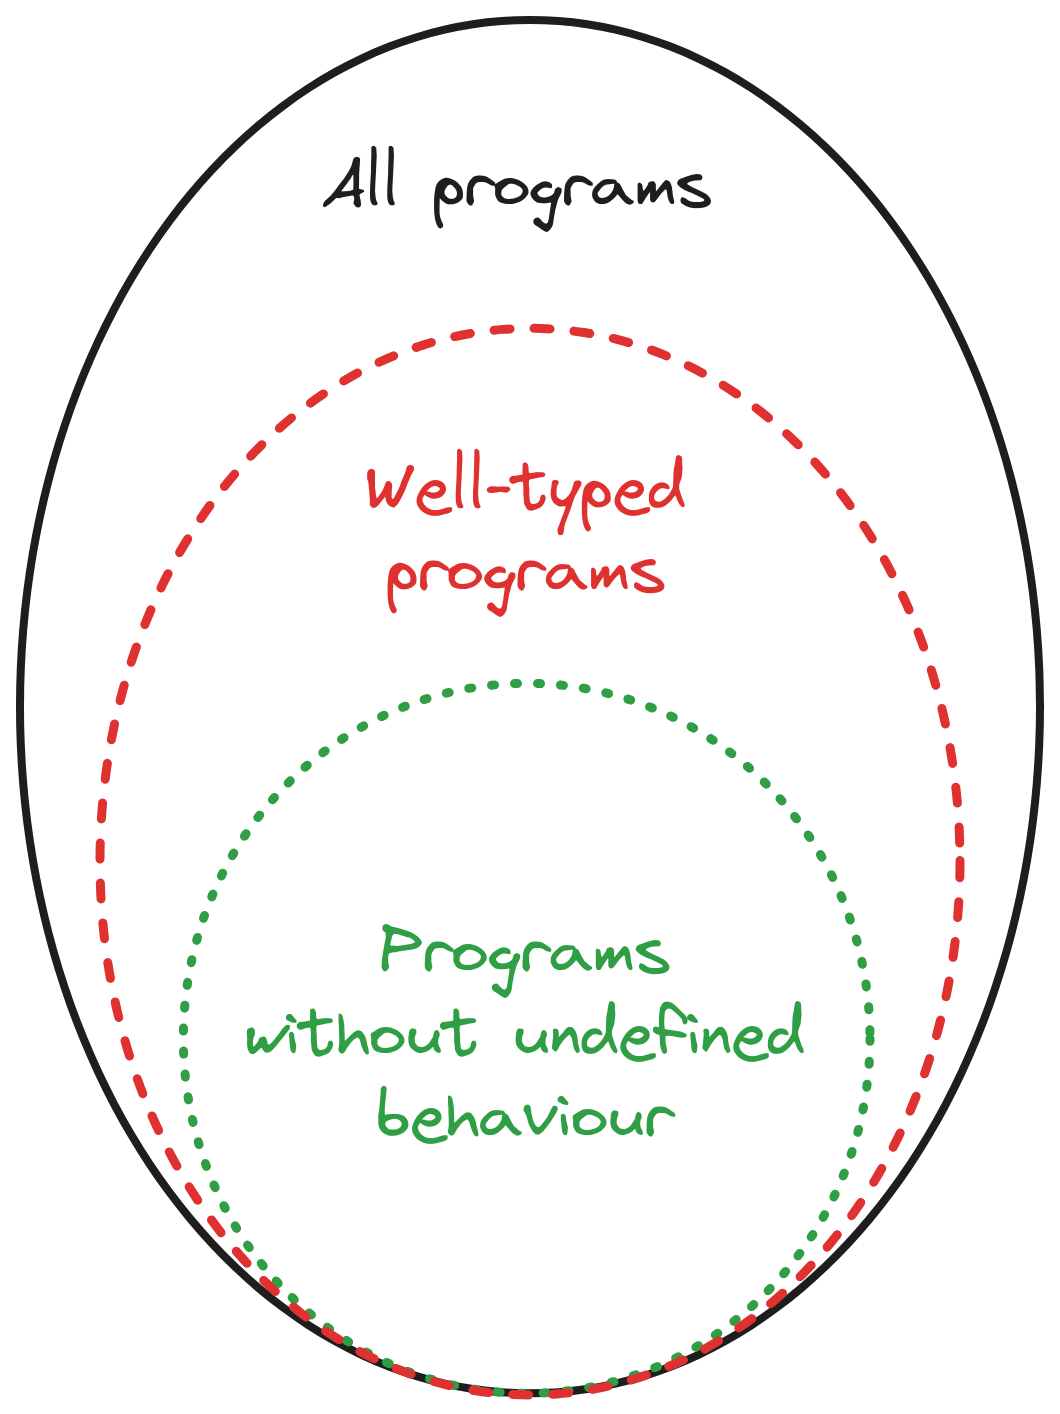
\includegraphics[width=0.5\textwidth]{images/3_translation/excalidraw_programs_venn.png}
    \caption{A diagram to show the relative powers of increasingly restrictive program models.}
    \label{fig:excalidraw_programs_venn}
\end{figure}

When translating from languages such as C++ which allow undefined behaviour to Rust which prohibits it by default, there are additional challenges beyond just reconciling the abstractions of the program models to express the same functionality. There are fewer safe Rust programs than C++ programs, and as a result a direct mapping to Rust may not exist if the program relies on undefined behaviour. In this case, the translation must either leverage the \mintinline{rust}{unsafe} keyword to allow such behaviour, or use a different, safe, mechanism to express the same functionality.


\subsection{Overview of HPCCG}
\label{sec:overview-hpccg}

As discussed in the background to HPCCG in section \ref{ssec:hpccg}, the dominant computation kernel is an implementation of sparse matrix-vector multiplication. In addition to this, there are two other kernels, the vector dot product and pairwise summation of two scaled vectors. To facilitate performant implementation of these operations, HPCCG uses a pointer based implementation of the Yale format to represent sparse matrices, which is explained in detail in Appendix \ref{sec:hpccg-sparse-matrix-appendix}.

Unfortunately, this pointer based implementation presents difficulties when translating to Rust, as operations on raw pointers considered unsafe, as the borrower checker is less able to reason about their memory safety. This difficulty is addressed in the first two translation versions, \ref{sec:translation-direct} and \ref{sec:translation-direct}.

\section{Implementation}
\label{sec:translation-implementation}

This section provides a description of the technical details of the translation process.
% In order to guarantee that the Rust implementation is performant as possible, and hence representative of the capabilities of the Rust language, a workflow of incremental improvement was adopted for the translation process.
First, a direct translation to Rust was undertaken, matching the program model as closely as possible to provide confidence in program equivalence. Then, a number of incremental improvements to the Rust implementation were undertaken to result in a performant serial implementation of the HPCCG mini-app. Finally, this serial implementation was modified to implement shared and distributed memory parallelism using \texttt{rayon} and the Rust MPI bindings. Source code for each of these translation versions can be found in the \texttt{hpccg-rs} \texttt{git} repository.


\subsection{Direct translation}
\label{sec:translation-direct}
The first translation was designed to be as direct a mapping between the program models of C++ and Rust as possible. This helped develop a strong understanding of the codebase, and gave initial confidence in program equivalence, as the only factor which could result in different program functionality was the language semantics of Rust differing from C++.

% In C++, pointers are very commonly used for memory indirection. This is especially true i
In C++ codebases for High-Performance Computing, memory indirection using pointers is very common. This is because such codebases often operate on multi-dimensional arrays representing meshes, which are represented in C++ by pointers. However, using pointers in this way makes programs very susceptible to a certain category of bugs, for example accessing uninitialised memory as a result of faulty pointer arithmetic. As discussed in \Cref{ch:background}, interaction with raw pointers in Rust is considered an \mintinline{rust}{unsafe} operation, as it is difficult to statically guarantee that it will not result in undefined behaviour. Much of the behaviour of pointers can instead be implemented in Rust through borrowing references, but strict ownership rules prohibit some common behaviour such as concurrent mutable references, requiring the use of smart pointers.

This presented the first significant challenge in the translation effort, as the implementation of the Yale representation of sparse matrix in HPCCG relies heavily on raw pointers and pointer arithmetic. This complicates the direct translation process, as references and smart pointers in Rust necessarily have different semantics to raw pointers, and may be less performant. This was identified as a risk during the specification phase, and was captured in the Risk Matrix \ref{tab:risk_matrix}, which is shown in \Cref{ch:project-management} in the discussion of project management. A truncated version of the data structure which implements this Yale representation in C++ is shown in Listing \ref{listing:cpp-sparse-matrix-structure}.

\begin{code}
    %TC:ignore
    \begin{minted}{c++}
        struct HPC_Sparse_Matrix_STRUCT {
          int total_nrow;
          long long total_nnz;
          int  * nnz_in_row;
          double ** ptr_to_vals_in_row;
          int ** ptr_to_inds_in_row;
          double *list_of_vals;
          int *list_of_inds;
        }
    \end{minted}
    %TC:endignore
    \caption{A truncated version of the C++ data structure which implements the Yale representation of the sparse matrix, from Heroux's original implementation of HPCCG \cite{MantevoHPCCG2023}.}
    \label{listing:cpp-sparse-matrix-structure}
\end{code}

% This data structure must then be populated to the initial configuration of the conjugate gradient problem, with the reference C++ implementation shown in Listing \ref{listing:cpp-sparse-matrix-structure-population}. This process presents a challenge to the translation process, not only because it dereferences raw pointers, but also it violates Rust's ownership rules, as there are concurrent mutable and immutable pointers to the data, for example lines 7 and 17 in Listing \ref{listing:cpp-sparse-matrix-structure-population}.

% \begin{code}
%     %TC:ignore
%     \begin{minted}{c++}
% for (int iz=0; iz<nz; iz++) {
%     for (int iy=0; iy<ny; iy++) {
%         for (int ix=0; ix<nx; ix++) {
%         int curlocalrow = iz*nx*ny+iy*nx+ix;
%         int currow = start_row+iz*nx*ny+iy*nx+ix;
%         int nnzrow = 0;
%         (*A)->ptr_to_vals_in_row[curlocalrow] = curvalptr;
%         (*A)->ptr_to_inds_in_row[curlocalrow] = curindptr;
%         for (int sz=-1; sz<=1; sz++) {
%             for (int sy=-1; sy<=1; sy++) {
%                 for (int sx=-1; sx<=1; sx++) {
%                     int curcol = currow+sz*nx*ny+sy*nx+sx;
%                         if ((ix+sx>=0) && (ix+sx<nx) && (iy+sy>=0) && (iy+sy<ny) && (curcol>=0 && curcol<total_nrow)) {
%                             if (!use_7pt_stencil || (sz*sz+sy*sy+sx*sx<=1)) {
%                                 if (curcol==currow) {
%                                     *curvalptr++ = 27.0;
%                                 } else {
%                                     *curvalptr++ = -1.0;
%                                 }
%                                 *curindptr++ = curcol;
%                                 nnzrow++;
%                             } 
%                         }
%                 }
%             }
%         }
%         (*A)->nnz_in_row[curlocalrow] = nnzrow;
%         nnzglobal += nnzrow;
%         (*x)[curlocalrow] = 0.0;
%         (*b)[curlocalrow] = 27.0 - ((double) (nnzrow-1));
%         (*xexact)[curlocalrow] = 1.0;
%         }
%     }
% }
%     \end{minted}
%     %TC:endignore
%     \caption{A truncated version of the C++ function to populate the initial configuration of the sparse matrix, from Heroux's original implementation of HPCCG \cite{MantevoHPCCG2023}.}
%     \label{listing:cpp-sparse-matrix-structure-population}
% \end{code}

% This code snippet exemplifies how HPCCG is not a single computational kernel, nor a toy example, but a mini-app representative of structural complexities in full-scale applications for High-Performance Computing.

The first key insight in the translation process is that the interior mutability pattern of smart pointers, discussed in section 15-5 of the Rust book \cite{RustProgrammingLanguage} can be used to represent this functionality, despite the presence of concurrent mutable and immutable pointers to the data. Instead of arrays of pointers such as \mintinline{c++}{int ** ptr_to_inds_in_row} as shown in Listing \ref{listing:cpp-sparse-matrix-structure}, the \mintinline{rust}{Rc<RefCell<f64>>} construct can be used to create a vector of items which allow concurrent mutable and immutable borrows. This presents a safe interface to an \mintinline{rust}{unsafe} implementation which performs checks at runtime to guarantee memory safety. As such, the data structure shown in Listing \ref{listing:cpp-sparse-matrix-structure} can be re-written in Rust, as shown in Listing \ref{listing:rust-sparse-matrix-structure}.

\begin{code}
    %TC:ignore
    \begin{minted}{rust}
        struct SparseMatrix {
            pub total_nrow: i32,
            pub total_nnz: i32,
            pub nnz_in_row: Vec<i64>,
            pub ptr_to_vals_in_row: Vec<Rc<RefCell<f64>>>,
            pub ptr_to_inds_in_row: Vec<Rc<RefCell<i32>>>,
            pub list_of_vals: Vec<Rc<RefCell<f64>>>,
            pub list_of_inds: Vec<Rc<RefCell<i32>>>,
        }
    \end{minted}
    %TC:endignore
    \caption{A truncated version of the sparse matrix data structure, directly translated to Rust using the interior mutability pattern of smart pointers.}
    \label{listing:rust-sparse-matrix-structure}
\end{code}

%% MOVED LATER!
% As discussed in \Cref{ch:background}, the dominant computational kernel of HPCCG is sparse matrix-vector computation. Listing \ref{} shows how this is implemented leveraging the Yale sparse matrix representation outlined in Listing \ref{listing:cpp-sparse-matrix-structure}.
%% MOVED LATER!
% \begin{code}
%     %TC:ignore
%     \begin{minted}{c++}
% int HPC_sparsemv( HPC_Sparse_Matrix *A, const double * const x, double * const y) {
%   const int nrow = (const int) A->local_nrow;
%   for (int i=0; i< nrow; i++) {
%       double sum = 0.0;
%       const double * const cur_vals = 
%      (const double * const) A->ptr_to_vals_in_row[i];
%       const int    * const cur_inds = 
%      (const int    * const) A->ptr_to_inds_in_row[i];
%       const int cur_nnz = (const int) A->nnz_in_row[i];
%       for (int j=0; j< cur_nnz; j++) {
%         sum += cur_vals[j]*x[cur_inds[j]];
%       }
%       y[i] = sum;
%     }
%   return(0);
% }
%     \end{minted}
%     %TC:endignore
%     \caption{The C++ function to compute sparse matrix-vector multiplication, from Heroux's original implementation of HPCCG \cite{MantevoHPCCG2023}.}
%     \label{listing:cpp-sparsemv}
% \end{code}

% Having implemented the data structure leveraging the interior mutability pattern as shown in Listing \ref{listing:rust-sparse-matrix-structure}, this sparse matrix-vector kernel can be translated to Rust, as shown in Listing \ref{listing:rust-sparsemv-direct}. Here, we can see the structural similarities between the original code and the translation, but also instances where smart pointers introduce extra boilerplate, such as the \mintinline{rust}{borrow} function on lines 9 and 10.

% \begin{code}
%     \begin{minted}[linenos,breaklines]{rust}
% pub fn sparsemv(matrix: &SparseMatrix, vector: &[f64]) -> Vec<f64> {
%     let nrow = matrix.local_nrow as usize;
%     let mut y = Vec::with_capacity(vector.len());
%     let mut start_index = 0;
%     for i in 0..nrow {
%         let mut sum = 0.0;
%         let cur_nnz = matrix.nnz_in_row[i] as usize;
%         for j in 0..cur_nnz {
%             let val = *matrix.list_of_vals[start_index + j].borrow();
%             let ind = *matrix.list_of_inds[start_index + j].borrow() as usize;
%             sum += val * vector[ind];
%         }
%         y.push(sum);
%         start_index += cur_nnz;
%     }
%     y
% }
%     \end{minted}
%     \caption{A direct translation to Rust of the C++ function to compute sparse matrix-vector multiplication.}
%     \label{listing:rust-sparsemv-direct}
% \end{code}

%% MOVED LATER!
% There are two other computational kernels in HPCCG: calculating a vector dot product, and pairwise summation of two scaled vectors. However, as discussed in \Cref{ch:background}, these take up a much smaller proportion of the runtime than the sparse matrix-vector multiplication. In addition to this, they present significantly less challenge with respect to translation, as they are dependent only on C++ arrays which can be implemented in Rust through the \mintinline{rust}{Vec} type, rather than a custom data structure of pointers as with the sparse matrix representation.

Unfortunately, leveraging the interior mutability pattern comes at a steep cost to performance, as the guarantees against undefined behaviour are deferred to runtime, meaning every pointer dereference must be bounds checked, doubling the instruction count per dereference.
% This can be seen in Figure \ref{fig:perf_annot_labelled}, which shows a screenshot of the \texttt{perf} performance profiler, which is introduced in more depth in \ref{ssec:perf profiler}.
% \begin{figure}[H]
%     \centering
%     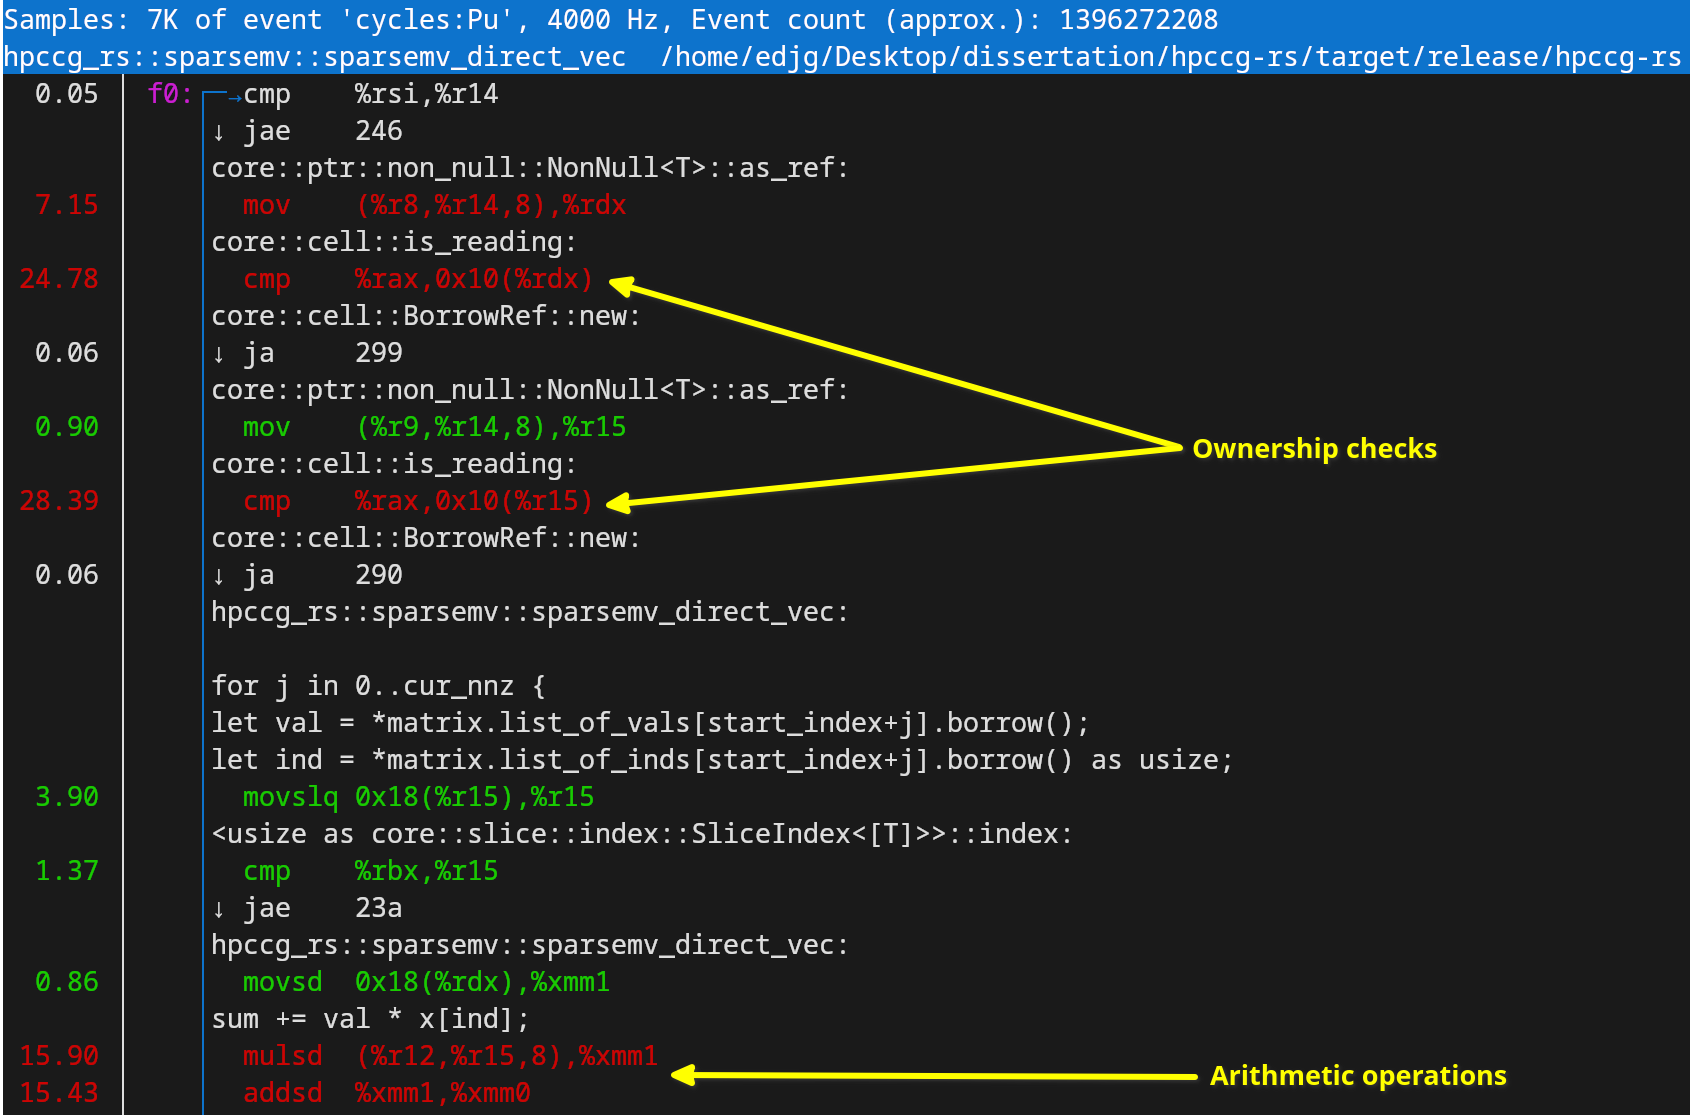
\includegraphics[width=0.75\textwidth]{images/3_translation/perf_annot_labelled.png}
%     \caption{An annotated screenshot of the \texttt{perf} performance profiler, showing the dominating performance impact of extra instructions checking the dereference operation.}
%     \label{fig:perf_annot_labelled}
% \end{figure}
This severe performance cost is unacceptable for High-Performance Computing use cases. Hence, for Rust to be viable for these purposes, there must be a way to avoid incurring this cost.

\subsection{Reworked data structure}
\label{sec:translation-reworked-data-structure}

Having written a direct translation of HPCCG into Rust, the next step was to incrementally improve it by modifying the implementation to use a data structure more amenable to Rust's program model.
% In Rust, there are many constraints placed on the use of pointers, due to the difficulty to reason about them and their memory safety at compile time.
In HPCCG, pointers are used only to define and refer to items within arrays. In addition to this, there are fewer semantic restrictions on indexes in Rust than raw pointers or borrowed references, as they are restricted to the specific domain of accessing arrays, rather than the many use cases pointers support. As a result of this, it was decided to re-work the Yale representation data structure of the sparse matrix to use indexing as opposed to pointers.

% As part of its rich type system, the Rust language provides a data type specific to data used as indexes, called \mintinline{rust}{usize}. The amount of data stored by this type depends on the address space of the machine it is compiled on, with 32-bit architectures having the same domain as the \mintinline{rust}{u32} -- an unsigned 32 bit integer, and 64-bit architectures having the same domain as \mintinline{rust}{u64}. This guarantees that any length of array can be indexed by this type, but also differentiates data which is used as an index from other data, allowing developers to more intuitively understand the meaning of code through its type system.

% This switch from a pointer to index based implementation of the sparse matrix data structure is shown in Listing \ref{listing:rust-sparse-matrix-structure-indexed}, contrasting the direct Rust translation shown in Listing \ref{listing:rust-sparse-matrix-structure}.This change also reduces the complexity of the implementation to populate the initial configuration of the sparse matrix. In the index based structure, only the vector \mintinline{rust}{push} and indexing operations are required, whereas the direct translation using smart pointers also requires careful use of the \mintinline{rust}{borrow_mut} and \mintinline{rust}{clone} operations. This reduces the total wall time required to run the program, which includes the time to populate the initial configurations for the mini-app.

In addition to this, a second key insight is that the pointers in the \mintinline[breaklines,breakafter=\_]{c++}{ptr_to_vals_in_row} and \mintinline[breaklines,breakafter=\_]{c++}{ptr_to_inds_in_row} refer to the same indices in arrays at different memory addresses. As a result of this, only a single vector of indices is required, rather than two arrays of pointers. This slightly reduces the memory bandwidth required to transfer the sparse matrix, which may increase performance in memory-bound workloads, as characterised by the roofline plots shown \Cref{ch:performance}. The final incremental improvement of the data structure using a single vector of indices is shown in Listing \ref{listing:rust-sparse-matrix-structure-indexed}.

\begin{code}
    %TC:ignore
    \begin{minted}{rust}
        struct SparseMatrix {
            pub total_nrow: usize,
            pub total_nnz: usize,
            pub nnz_in_row: Vec<usize>,
            pub row_start_inds: Vec<usize>,
            pub list_of_vals: Vec<f64>,
            pub list_of_inds: Vec<usize>,
        }
    \end{minted}
    %TC:endignore
    \caption{A truncated version of the sparse matrix data structure, re-worked in Rust to use an index rather than pointer based implementation of the Yale representation.}
    \label{listing:rust-sparse-matrix-structure-indexed}
\end{code}

Since High-Performance Computing workloads are often array or mesh based, this strategy of replacing pointers with indices still holds for the dominant computational kernels of many full applications. Where pointers cannot be substituted with indices, borrowed references should be preferred, then smart pointers such as the \mintinline{rust}{Rc<RefCell<f64>>} construct as a worst-case solution.

As discussed in \Cref{ch:background}, the dominant computational kernel of HPCCG is sparse matrix-vector computation. Listing \ref{} shows how this is implemented leveraging the Yale sparse matrix representation outlined in Listing \ref{listing:cpp-sparsemv}. Listing \ref{listing:rust-sparsemv-indexed} shows how this kernel can be translated using the indexed data structure as a point of reference for later changes.

\begin{code}
    %TC:ignore
    \begin{minted}{rust}
        fn sparsemv(matrix: &SparseMatrix, vector: &[f64]) -> Vec<f64> {
            let nrow = matrix.local_nrow;
            let mut result = Vec::with_capacity(vector.len());
            for i in 0..nrow {
                let mut sum = 0.0;
                let start_ind = matrix.row_start_inds[i];
                let cur_nnz = matrix.nnz_in_row[i];
                for j in 0..cur_nnz {
                    sum += matrix.list_of_vals[start_ind + j]
                        * vector[matrix.list_of_inds[start_ind + j]];
                }
                result.push(sum);
            }
            result
        }
    \end{minted}
    %TC:endignore
    \caption{A translation to Rust of the C++ function, using a single-indexed sparse matrix representation to compute sparse matrix-vector multiplication.}
    \label{listing:rust-sparsemv-indexed}
\end{code}

There are two other computational kernels in HPCCG: calculating a vector dot product, and pairwise summation of two scaled vectors. However, as discussed in \Cref{ch:background}, these take up a much smaller proportion of the runtime than the sparse matrix-vector multiplication. In addition to this, they present significantly less challenge with respect to translation, as they are dependent only on C++ arrays which can be implemented in Rust as vectors, rather than a custom data structure of pointers as with the sparse matrix representation.

\subsection{Bounds checking}
\label{sec:translation-bounds-checking}

In Rust, all array indexing operations are bounds checked by default, to guarantee memory safety. This incurs a performance cost as a result of this comparison operation, and any resultant pipeline stalls as a result of it. As a result of this, the default indexing strategy in Rust is around twice as slow as in languages without these checks, such as C++. This result is explained in depth \Cref{ch:performance}, as part of a discussion of the \texttt{perf} performance profiler.

Fortunately, Rust provides a mechanism to disable these runtime checks -- the \mintinline{rust}{get_unchecked} function on vectors. However, this function is necessarily \mintinline{rust}{unsafe}, as it could result in accessing uninitialised memory if the programmer provides an index beyond the size of the vector. Listing \ref{listing:rust-sparsemv-unchecked} shows how the implementation of the sparse matrix-vector multiplication kernel can be modified to avoid runtime bounds checking.

\begin{code}
    %TC:ignore
    \begin{minted}[firstnumber=6]{rust}
        let start_ind = unsafe { *matrix.row_start_inds.get_unchecked(i) };
        let cur_nnz = unsafe { *matrix.nnz_in_row.get_unchecked(i) };
        for j in 0..cur_nnz {
            sum += unsafe {
                matrix.list_of_vals.get_unchecked(
                    start_ind + j
                )
                    *
                vector.get_unchecked(
                    *matrix.list_of_inds.get_unchecked(
                        start_ind + j
                    )
                )
            };
        }
    \end{minted}
    %TC:endignore
    \caption{A translation to Rust of the C++ function, using unchecked vector indexing to compute sparse matrix-vector multiplication.}
    \label{listing:rust-sparsemv-unchecked}
\end{code}

However, this approach nullifies Rust's beneficial property of guaranteeing memory safety. We are disabling runtime checks of indexes to gain performance, and hence regressing back to C++ with the only guarantees of memory safety being through programmer confidence. However, the Rust language provides syntax sugars in the form or zero-cost abstractions which can help avoid these unsafe operations in common use cases.

\subsection{Iterators}
\label{sec:translation-iterators}

Along with its rich type system, iterators are one of the places where the influence of functional languages on Rust is most clear. Functions such as \texttt{map}, \texttt{zip}, and \texttt{fold} process streams of data, taking inline functional closures as arguments to define their behaviour. This style of programming is particularly amenable to memory safety, as functions such as \texttt{map} typically operate on a single stream of data, avoiding the problem of holding multiple mutable references.

A key feature of Rust is zero-cost abstractions. Ibrahim Dursun describes this as ``your flavour of code doesn’t affect the performance. It doesn’t matter if you use loops or closures, they all compile down to the same assembly'' \cite{RustZeroCost2020}. Iterators are a common example of such zero-cost abstractions, as they provide a syntactic sugar for writing common list operations in a functional way which compiles down to at least equally performant assembly as a simple loop. In fact, iterators can provide a performance benefit over looping through and individually indexing a vector. Since the length of the list being processed is known within the iterator abstraction, it can guarantee that its indexing operations are within bounds. This allows it to perform \mintinline{rust}{unsafe} unchecked indexing internally whilst still providing a safe API externally.

As such, the sparse matrix-vector multiplication can be re-written to leverage the iterator design pattern, as shown in Listing \ref{listing:rust-sparsemv-iterator}. This significantly deviates in structure from the original C++ and previous Rust implementations, replacing the outer loop of the kernel with an iterator which maps a functional closure over values in the matrix.

\begin{code}
    %TC:ignore
    \begin{minted}{rust}
fn sparsemv(matrix: &SparseMatrix, vector: &[f64]) -> Vec<f64> {
    matrix.row_start_inds.iter()
        .zip(matrix.nnz_in_row.iter())
        .map(|(&start_ind, &cur_nnz)| {
                let mut sum = 0.0;
                for j in 0..cur_nnz {
                    sum += unsafe {
                        matrix.list_of_vals.get_unchecked(
                            start_ind + j
                        )
                            *
                        vector.get_unchecked(
                            *matrix.list_of_inds.get_unchecked(
                                start_ind + j
                            )
                        )
                    };
                }
                sum
            }
        ).collect()
}
    \end{minted}
    %TC:endignore
    \caption{A translation to Rust of the C++ function, using iterators to compute sparse matrix-vector multiplication.}
    \label{listing:rust-sparsemv-iterator}
\end{code}

Although in this case the use of iterators does not eliminate the need for unchecked array indexing, it reduces the number of instances of their use, which reduces the surface for possible invalid memory access within a program. It is possible to construct nested iterators such that only one unchecked index operation is required -- which cannot be removed as it is part of the data in the sparse matrix representation, and doesn't range over a known set of values. However, this was not done in this implementation to make the implementation more amenable to the use of \texttt{rayon} for shared memory parallelism.

\subsection{Shared memory parallelism}
\label{sec:translation-rayon}

\Cref{ch:background} introduces Rust as facilitating ``Fearless Concurrency'' through its language design. Having modified the Rust implementation to use iterators, it is incredibly easy to leverage shared memory parallelism through \texttt{rayon}. The only change required is replacing instances of the native Rust \texttt{iter} function with the \texttt{par\_iter} function provided by \texttt{rayon}. As such, the sparse matrix-vector multiplication kernel can be implemented as shown in Listing \ref{listing:rust-sparsemv-rayon}.

\begin{code}
    %TC:ignore
    \begin{minted}{rust}
        use rayon::prelude::*;
        
        pub fn sparsemv(matrix: &SparseMatrix, vector: &[f64]) -> Vec<f64> {
            matrix.row_start_inds.par_iter()
                .zip(matrix.nnz_in_row.par_iter())
                .map(|(&start_ind, &cur_nnz)| {
                    // [snip]
                }).collect()
        }
    \end{minted}
    %TC:endignore
    \caption{A translation to Rust of the C++ function, using \texttt{rayon} to compute sparse matrix-vector multiplication using shared memory parallelism.}
    \label{listing:rust-sparsemv-rayon}
\end{code}

This change to leveraging shared memory parallelism requires only two eight characters to be changed -- adding the \texttt{par} prefix to the two outer zipped iterators. In addition to this, as a result of the Rust compiler's static checks, there are much stronger guarantees against data races. Section \ref{ssec:shared-memory-paralellism} of \Cref{ch:background} showed how easy it is to introduce a data race using OpenMP even for a trivial example. However, the ownership constraints and scoping rules of closures for functions over iterators ensure that data cannot be concurrently accessed across threads. The combination of these two factors, ease of switching to multi-threading and guarantees of correctness, empowers developers to quickly write performant code by leveraging shared memory parallelism.

The use of packages such as \texttt{rayon} allows developers to write multi-threaded Rust code incredibly quickly, and with confidence in its correctness. Due to the current trend in hardware design towards multi-processor architectures in machines discussed in \Cref{ch:background}, this allows developers to fully leverage the performance of commodity hardware, which is crucial in a High-Performance Computing context.

\subsection{Distributed memory parallelism}
\label{sec:translation-mpi}

\Cref{ch:background} introduced MPI as a standard for distributed memory parallelism with implementations in languages such as C++, FORTRAN and Java. Unfortunately, Rust is notable in its absence from this list of languages with MPI implementations. However, a key feature of Rust is its support for foreign function interfaces, allowing it to invoke functions implemented in other languages. This means that a Rust can bind into a C++ implementation of MPI using a foreign function interface, then provide a safe API over these bindings. The \texttt{mpi} crate \cite{noauthor_rsmpirsmpi_2024} %\cite{RsmpiRsmpi2024}
provides these bindings, along with an idiomatic interface around them.

The process of translating the MPI aspect of HPCCG into Rust was by far the most difficult part of the translation process. It was significantly more complex than the next most difficult aspect of populating the data structure -- alone taking around two weeks dedicated work. This difficulty was broadly as a result of three key factors:

\begin{enumerate}
    \item The length of the codebase to translate -- the \texttt{make\_local\_matrix.cpp} file alone is 612 lines long
    \item The imperfect mapping between the C++ MPI calls and the Rust MPI bindings
    \item The minimal documentation of the Rust MPI bindings
\end{enumerate}

An example of one of these difficulties is in both the final stage of making the local matrix and the operation to exchange external data between ranks each iteration, there is an MPI idiom which maps particularly poorly to Rust.
The example of this of exchanging data between ranks is shown in Listing \ref{listing:cpp-mpi-exchange-externals}.

\begin{code}
    %TC:ignore
    \begin{minted}{c++}
int MPI_MY_TAG = 99;  
MPI_Request * request = new MPI_Request[num_neighbors];
double *x_external = (double *) x + local_nrow;

// Post receives first 
for (i = 0; i < num_neighbors; i++) {
    int n_recv = recv_length[i];
    MPI_Irecv(x_external, n_recv, MPI_DOUBLE, neighbors[i], MPI_MY_TAG, 
    MPI_COMM_WORLD, request+i);
    x_external += n_recv;
}

// Fill up send buffer
for (i=0; i<total_to_be_sent; i++) {
    send_buffer[i] = x[elements_to_send[i]];
}

// Send to each neighbor
for (i = 0; i < num_neighbors; i++) {
    int n_send = send_length[i];
    MPI_Send(send_buffer, n_send, MPI_DOUBLE, neighbors[i], MPI_MY_TAG, 
    MPI_COMM_WORLD);
    send_buffer += n_send;
}

// Complete the reads issued above
MPI_Status status;
for (i = 0; i < num_neighbors; i++) {
    if ( MPI_Wait(request+i, &status) ) {
        cerr << "MPI_Wait error\n"<<endl;
        exit(-1);
    }
}
    \end{minted}
    %TC:endignore
    \caption{A code snippet from the C++ implementation to exchange external mesh data between MPI ranks, from Heroux's original implementation of HPCCG \cite{MantevoHPCCG2023}.}
    \label{listing:cpp-mpi-exchange-externals}
\end{code}

It is exceedingly difficult to reason about this idiom's memory and concurrent safety properties. This is because first a arbitrary number of asynchronous receive operations known only at runtime are spawned, each of which receive data into a location in a buffer again known only at runtime. After this, data is sent to these receive operations, relying on program logic to ensure no asynchronous receive operations are left waiting for a response. If this logic is faulty, the error would manifest as hanging indefinitely at the next MPI wait or barrier. This would be very difficult to debug, as the point in the codebase at which it hangs might be significantly displaced from the logic causing it to hang.

In order to implement this using the \texttt{mpi} crate, stronger guarantees about memory safety and tying together the sending and receiving operations are needed. This ensures that no asynchronous receive operations are left waiting for a response, and prevents data races. However, these strong guarantees are very difficult to achieve. The identified mechanism to implement this functionality in Rust is shown below in Listing \ref{listing:rust-mpi-exchange-externals}.

\begin{code}
    %TC:ignore
    \begin{minted}{rust}
let mpi_my_tag = 99;

let mut x_externals = vec![];
for i in 0..matrix.num_send_neighbors {
    let slice = vec![0.0; matrix.recv_length[i]];
    x_externals.push(slice);
}

// Fill up send buffer
for i in 0..matrix.total_to_be_sent {
    matrix.send_buffer[i] = vector[matrix.elements_to_send[i] as usize];
}

mpi::request::multiple_scope(matrix.num_send_neighbors, |scope, coll| {
    // Post receives first
    for (i, x_external) in x_externals.iter_mut().enumerate() {
        let rreq = world
            .process_at_rank(matrix.neighbors[i] as i32)
            .immediate_receive_into_with_tag(scope, x_external, mpi_my_tag);
        coll.add(rreq);
    }

    // Send to each neighbor
    let mut start = 0;
    for i in 0..matrix.num_send_neighbors {
        world
            .process_at_rank(matrix.neighbors[i] as i32)
            .send_with_tag(
                &matrix.send_buffer[start..start + matrix.send_length[i]],
                mpi_my_tag,
            );
        start += matrix.send_length[i];
    }
    
    // Complete the reads issued above
    while coll.incomplete() > 0 {
        coll.wait_any().expect("MPI_Wait error");
    }
});
    \end{minted}
    %TC:endignore
    \caption{A code snippet from the Rust translation to exchange external mesh data between MPI ranks.}
    \label{listing:rust-mpi-exchange-externals}
\end{code}

In the listing, we can see that populating the send buffer is moved out of the original order. This is required to conform to Rust's ownership rules, as the send buffer must be shared across the lexical scopes of multiple MPI requests defined in the closure on line 8. This helps resolve the memory safety concerns. In addition to this, we can see that the receive and send operations are paired within their scopes, which guarantees every asynchronous receive will receive data and not hang indefinitely.

Since the documentation for the \texttt{mpi} crate is very sparse, this translation was developed by reading the source code of the crate functions and their bindings into the C++ specification implementation, across many iterations trying to achieve the memory safety properties required for compilation.

In summary, it is possible to translate most existing C++ code using MPI into Rust with equivalent functionality using the \texttt{mpi} crate. However, this translation process is involved, requiring expertise which is hard to acquire due to the minimal documentation. As Rust and its ecosystem matures, this process is likely to get easier, with improved documentation and tweaks to the interface design.

% TODO: (+ poor documentation, link to future open source work)

\subsection{Performance comparison}
\label{sec:translation-performance}

% TODO: Could cut this as it partially duplicates later chapter?

In order to fairly assess the suitability of Rust for High-Performance Computing workloads, the translation of the mini-app being assessed must fully leverage the performance capabilities of Rust. As a result of this, the translation effort was driven by achieving performance, with each incremental improvement making progress towards this goal.

This section presents performance measurements, using the HPC MultiBench tool introduced in \Cref{ch:hpc-multibench}, of the total and individual kernel runtimes across the translations, and discusses the impact of the techniques applied on these results.

Figure \ref{fig:translations_total_line} provides an overall picture on how the different translations affect performance. It shows how the total wall time of each translation scales with the overall mesh size, making it clear that each incremental translation improves the performance of the mini-app as a whole, but with significant diminishing returns.

\begin{figure}[H]
    \centering
    % This file was created with tikzplotlib v0.10.1.
\begin{tikzpicture}

\definecolor{crimson2143940}{RGB}{214,39,40}
\definecolor{darkorange25512714}{RGB}{255,127,14}
\definecolor{darkslategray38}{RGB}{38,38,38}
\definecolor{forestgreen4416044}{RGB}{44,160,44}
\definecolor{lightgray204}{RGB}{204,204,204}
\definecolor{mediumpurple148103189}{RGB}{148,103,189}
\definecolor{steelblue31119180}{RGB}{31,119,180}

\begin{axis}[
axis line style={lightgray204},
height=0.45\textheight,
legend cell align={left},
legend style={
  fill opacity=0.8,
  draw opacity=1,
  text opacity=1,
  at={(0.03,0.97)},
  anchor=north west,
  draw=none
},
tick align=outside,
tick pos=left,
title={Rust Translations Total Times},
width=\textwidth,
x grid style={lightgray204},
xlabel=\textcolor{darkslategray38}{Mesh size},
xmajorgrids,
xmin=-650000, xmax=16400000,
xtick style={color=darkslategray38},
xtick={-2000000,0,2000000,4000000,6000000,8000000,10000000,12000000,14000000,16000000,18000000},
xticklabels={\ensuremath{-}0.2,0.0,0.2,0.4,0.6,0.8,1.0,1.2,1.4,1.6,1.8},
y grid style={lightgray204},
ylabel=\textcolor{darkslategray38}{Total time (s)},
ymajorgrids,
ymin=-31.8505937261743, ymax=685.76384916357,
ytick style={color=darkslategray38}
]
\path [draw=black, semithick]
(axis cs:125000,3.59458759136562)
--(axis cs:125000,3.64646240863438);

\path [draw=black, semithick]
(axis cs:1000000,29.8554891990788)
--(axis cs:1000000,30.2499108009212);

\path [draw=black, semithick]
(axis cs:3375000,100.220842202002)
--(axis cs:3375000,100.665007797998);

\path [draw=black, semithick]
(axis cs:8000000,246.437751474253)
--(axis cs:8000000,250.882798525747);

\path [draw=black, semithick]
(axis cs:15625000,636.8821391496)
--(axis cs:15625000,653.1450108504);

\path [draw=black, semithick]
(axis cs:125000,0.916547025389579)
--(axis cs:125000,0.922152974610421);

\path [draw=black, semithick]
(axis cs:1000000,6.92113850063032)
--(axis cs:1000000,6.94586149936968);

\path [draw=black, semithick]
(axis cs:3375000,24.2411972972584)
--(axis cs:3375000,24.7771527027416);

\path [draw=black, semithick]
(axis cs:8000000,63.0366056124052)
--(axis cs:8000000,64.7179943875948);

\path [draw=black, semithick]
(axis cs:15625000,125.655049885433)
--(axis cs:15625000,127.198900114567);

\path [draw=black, semithick]
(axis cs:125000,0.850320752802428)
--(axis cs:125000,0.855279247197572);

\path [draw=black, semithick]
(axis cs:1000000,6.55809995070753)
--(axis cs:1000000,6.62995004929247);

\path [draw=black, semithick]
(axis cs:3375000,22.8251515924216)
--(axis cs:3375000,23.4979984075784);

\path [draw=black, semithick]
(axis cs:8000000,60.4187811863453)
--(axis cs:8000000,60.8763688136547);

\path [draw=black, semithick]
(axis cs:15625000,118.750079255578)
--(axis cs:15625000,120.460770744422);

\path [draw=black, semithick]
(axis cs:125000,0.76824458699591)
--(axis cs:125000,0.77625541300409);

\path [draw=black, semithick]
(axis cs:1000000,6.19650354922889)
--(axis cs:1000000,6.31524645077111);

\path [draw=black, semithick]
(axis cs:3375000,21.7465944841671)
--(axis cs:3375000,22.3068055158329);

\path [draw=black, semithick]
(axis cs:8000000,56.9181220770364)
--(axis cs:8000000,58.3228779229636);

\path [draw=black, semithick]
(axis cs:15625000,113.696674820263)
--(axis cs:15625000,114.957775179737);

\path [draw=black, semithick]
(axis cs:125000,0.786085280220357)
--(axis cs:125000,0.795214719779643);

\path [draw=black, semithick]
(axis cs:1000000,6.2095920556317)
--(axis cs:1000000,6.3088579443683);

\path [draw=black, semithick]
(axis cs:3375000,21.8757629487399)
--(axis cs:3375000,22.0673870512601);

\path [draw=black, semithick]
(axis cs:8000000,58.8383344537454)
--(axis cs:8000000,59.2720155462546);

\path [draw=black, semithick]
(axis cs:15625000,114.237761390017)
--(axis cs:15625000,116.593888609983);

\addplot [semithick, steelblue31119180, mark=x, mark size=3, mark options={solid}]
table {%
125000 3.62052488327026
1000000 30.0527000427246
3375000 100.442924499512
8000000 248.660278320312
15625000 645.013549804688
};
\addlegendentry{Direct translation}
\addplot [semithick, darkorange25512714, mark=x, mark size=3, mark options={solid}]
table {%
125000 0.919350028038025
1000000 6.93349981307983
3375000 24.5091743469238
8000000 63.8773002624512
15625000 126.426971435547
};
\addlegendentry{Indexed translation}
\addplot [semithick, forestgreen4416044, mark=x, mark size=3, mark options={solid}]
table {%
125000 0.852800011634827
1000000 6.59402513504028
3375000 23.1615753173828
8000000 60.647575378418
15625000 119.605422973633
};
\addlegendentry{Single indexed translation}
\addplot [semithick, crimson2143940, mark=x, mark size=3, mark options={solid}]
table {%
125000 0.772249937057495
1000000 6.25587511062622
3375000 22.0266990661621
8000000 57.6204986572266
15625000 114.327224731445
};
\addlegendentry{No bounds checking translation}
\addplot [semithick, mediumpurple148103189, mark=x, mark size=3, mark options={solid}]
table {%
125000 0.790650010108948
1000000 6.2592248916626
3375000 21.9715747833252
8000000 59.05517578125
15625000 115.415824890137
};
\addlegendentry{Iterators translation}
\end{axis}

\end{tikzpicture}

    % 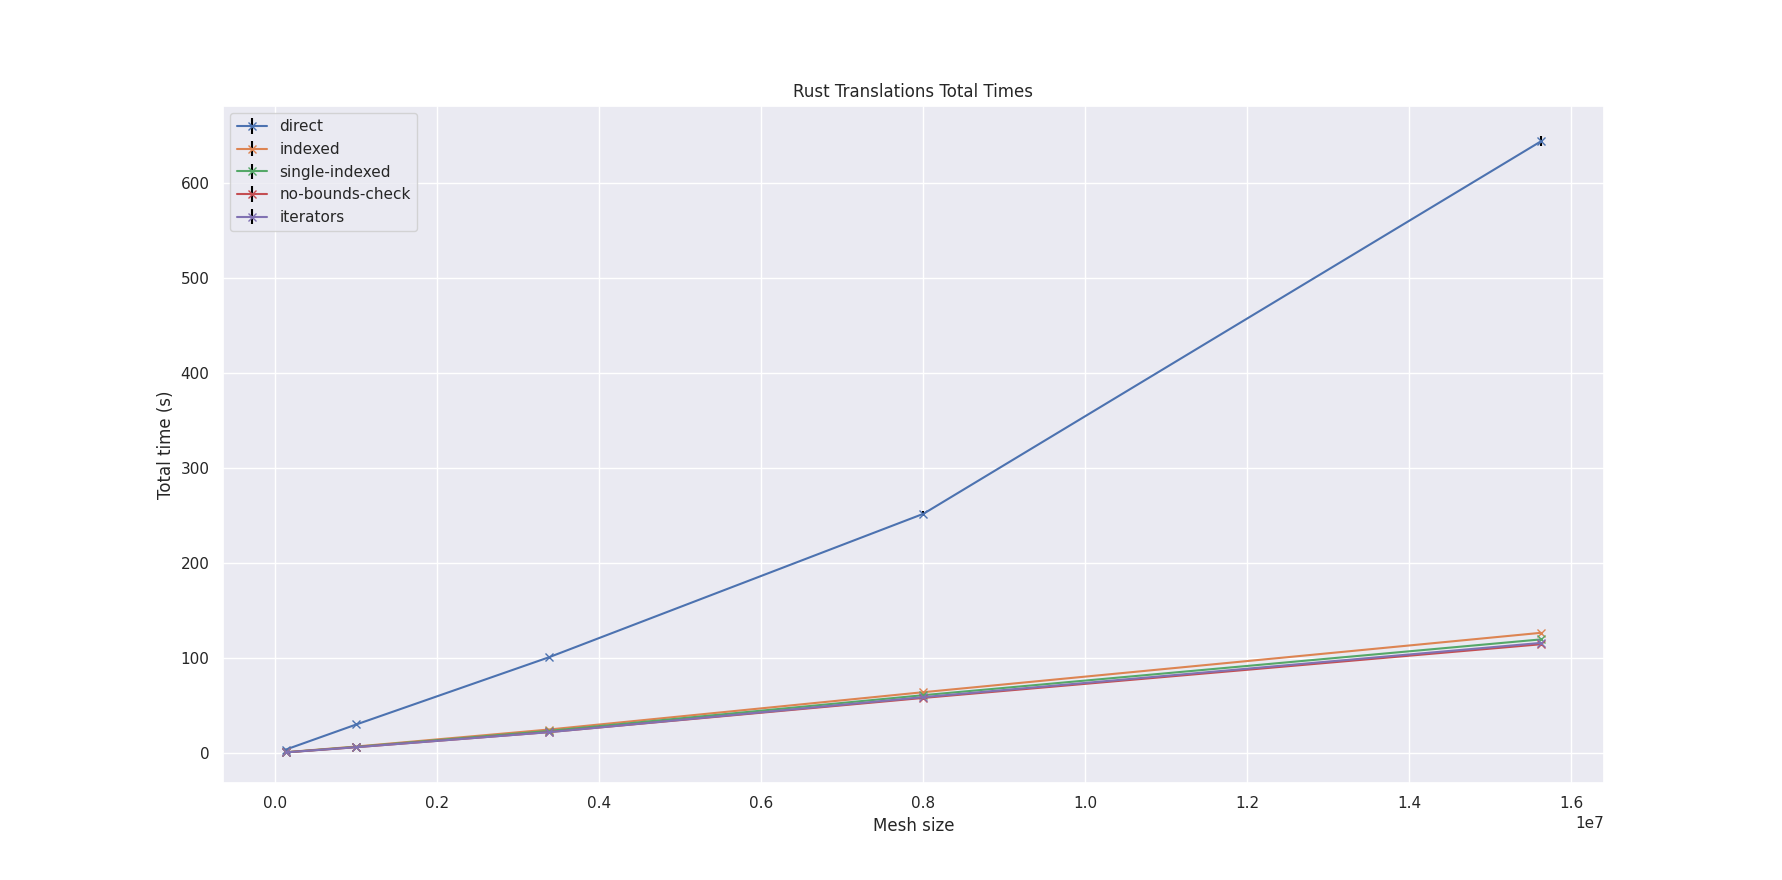
\includegraphics[width=\textwidth]{images/3_translation/performance/translations_total_line.png}
    \caption{A diagram showing the total wall time taken across the three kernels of each translation, as the overall mesh size is varied.}
    \label{fig:translations_total_line}
\end{figure}

% \begin{figure}[H]
%     \centering
%     % This file was created with tikzplotlib v0.10.1.
\begin{tikzpicture}

\definecolor{darkslategray38}{RGB}{38,38,38}
\definecolor{lavender234234242}{RGB}{234,234,242}
\definecolor{lightgray204}{RGB}{204,204,204}
\definecolor{peru22113282}{RGB}{221,132,82}
\definecolor{steelblue76114176}{RGB}{76,114,176}

\begin{axis}[
axis background/.style={fill=lavender234234242},
axis line style={white},
height=0.3\textheight,
legend cell align={left},
legend style={
  fill opacity=0.8,
  draw opacity=1,
  text opacity=1,
  draw=lightgray204,
  fill=lavender234234242
},
tick align=outside,
title={Multi-threaded Strong Scaling Plot},
width=\textwidth,
x grid style={white},
xlabel=\textcolor{darkslategray38}{Parallelisation degree},
xmajorgrids,
xmajorticks=false,
xmin=-0.55, xmax=33.55,
xtick style={color=darkslategray38},
y grid style={white},
ylabel=\textcolor{darkslategray38}{Wall time (s)},
ymajorgrids,
ymajorticks=false,
ymin=-1.61245177241997, ymax=37.6418579730152,
ytick style={color=darkslategray38}
]
\path [draw=black, semithick]
(axis cs:1,26.1187129070825)
--(axis cs:1,26.3012870929175);

\path [draw=black, semithick]
(axis cs:2,7.09681743392252)
--(axis cs:2,7.48818256607748);

\path [draw=black, semithick]
(axis cs:4,2.2880431416811)
--(axis cs:4,2.48695685831891);

\path [draw=black, semithick]
(axis cs:8,1.13491694260788)
--(axis cs:8,1.16008305739212);

\path [draw=black, semithick]
(axis cs:16,0.529226497308104)
--(axis cs:16,0.540773502691896);

\path [draw=black, semithick]
(axis cs:32,0.171835034190723)
--(axis cs:32,0.188164965809277);

\path [draw=black, semithick]
(axis cs:1,32.4324288335955)
--(axis cs:1,35.8575711664045);

\path [draw=black, semithick]
(axis cs:2,8.48762099922756)
--(axis cs:2,8.95237900077245);

\path [draw=black, semithick]
(axis cs:4,2.69217670016875)
--(axis cs:4,2.82782329983125);

\path [draw=black, semithick]
(axis cs:8,1.02137012440249)
--(axis cs:8,1.10362987559751);

\path [draw=black, semithick]
(axis cs:16,0.507925728922437)
--(axis cs:16,0.527074271077563);

\path [draw=black, semithick]
(axis cs:32,0.3525)
--(axis cs:32,0.3625);

\addplot [semithick, steelblue76114176, mark=x, mark size=3, mark options={solid}]
table {%
1 26.2099990844727
2 7.29250001907349
4 2.38750004768372
8 1.14750003814697
16 0.535000085830688
32 0.180000066757202
};
\addlegendentry{rust-rayon}
\addplot [semithick, peru22113282, mark=x, mark size=3, mark options={solid}]
table {%
1 34.1450004577637
2 8.72000026702881
4 2.75999999046326
8 1.0625
16 0.517499923706055
32 0.357499957084656
};
\addlegendentry{rust-rayon}
\end{axis}

\end{tikzpicture}

%     % 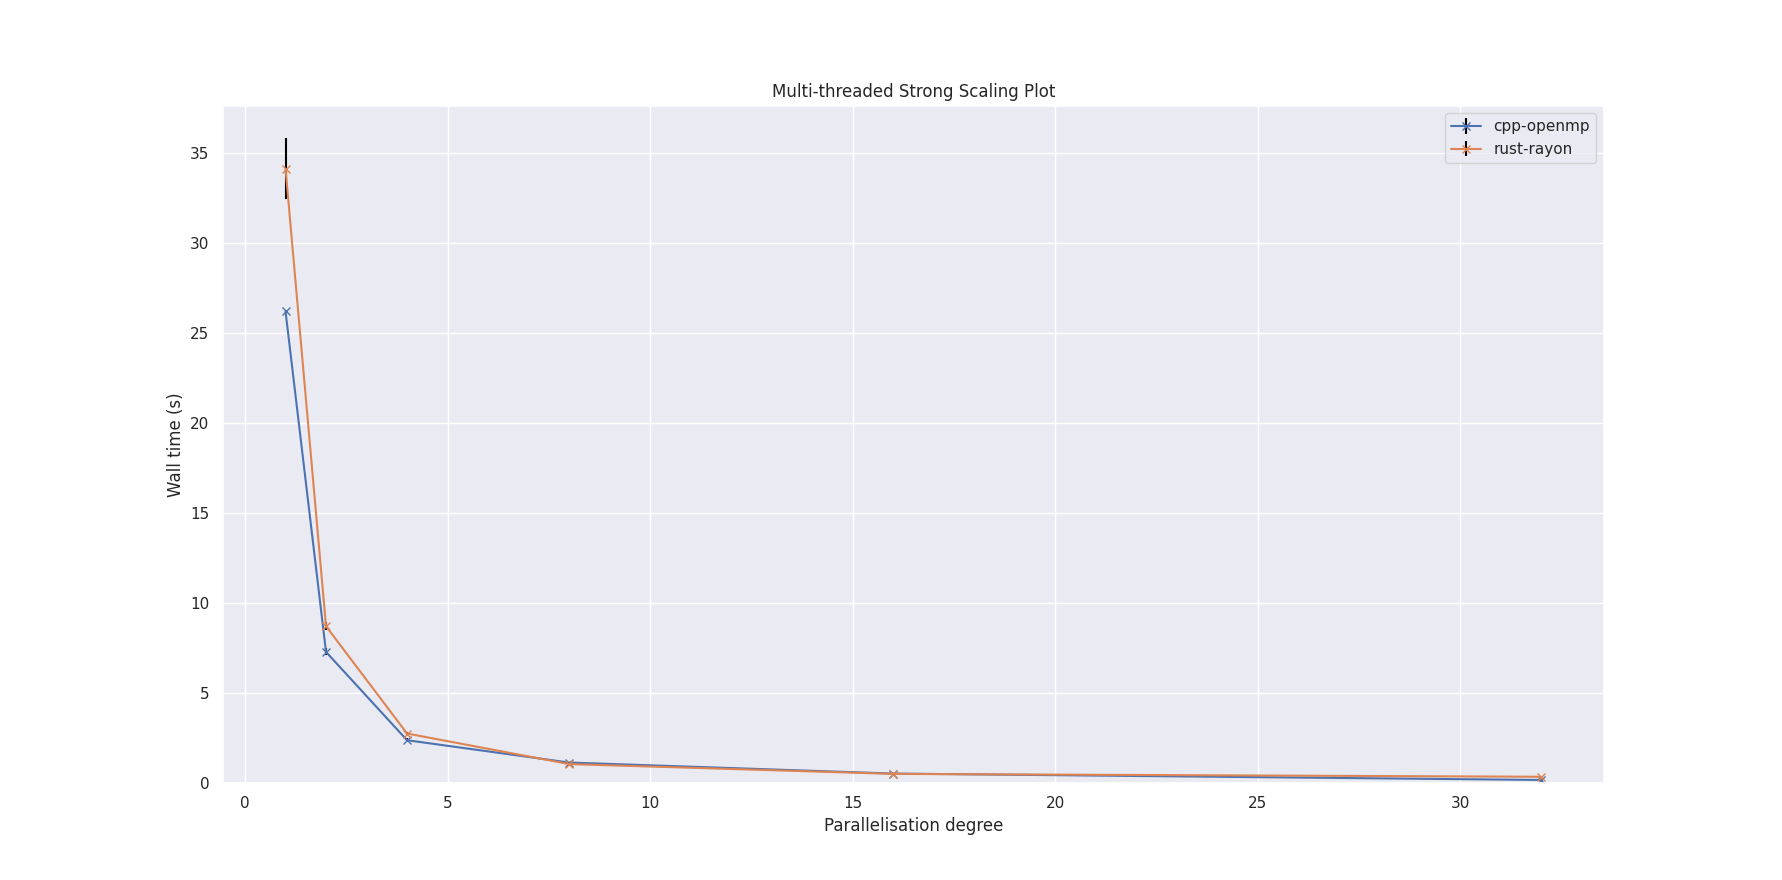
\includegraphics[width=\textwidth]{images/5_performance/scaling/strong_scaling_threaded.png}
%     \caption{A line plot comparing the strong scaling runtimes of the C++ and Rust implementations of HPCCG using shared memory parallelism.}
%     \label{fig:strong_scaling_threaded}
% \end{figure}


% Having seen the overall picture, we can analyse the performance of each kernel. The dominant kernel in the HPCCG mini-app is the sparse matrix-vector multiplication operation. We can see that the data structure refactor has a profound impact on performance here. The remaining kernels have a much smaller impact, with reducing the memory bandwidth required by adopting single indexing making a small improvement, then avoiding bounds checks or using iterators having very similar improvements in performance beyond that.

% \begin{figure}[H]
%     \centering
%     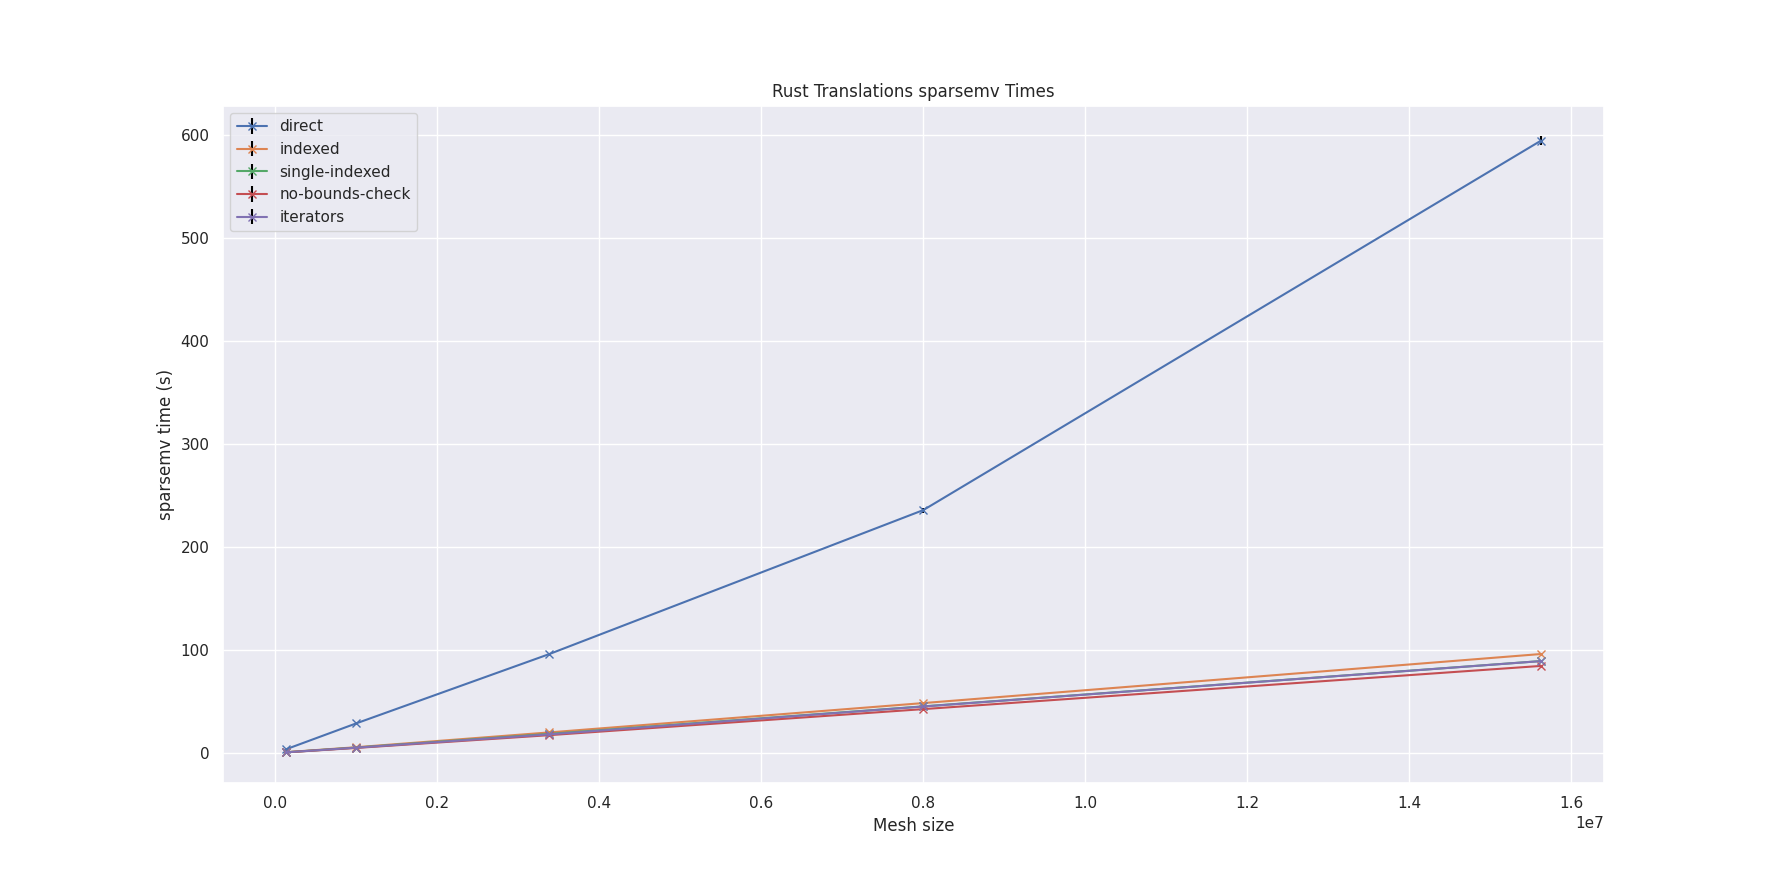
\includegraphics[width=\textwidth]{images/3_translation/performance/translations_sparsemv_line.png}
%     \caption{A diagram showing the wall time taken for the sparsmv kernel only of each translation, as the overall mesh size is varied.}
%     \label{fig:translations_waxpby_line}
% \end{figure}

% Figures \ref{fig:translations_ddot_line} and \ref{fig:translations_waxpby_line} show the wall time taken for the vector dot product and pairwise summation of two scaled vector kernels respectively. As compared with the sparse matrix-vector kernel, shown in Figure \ref{fig:translations_waxpby_line}, they are much less affected by data structure refactoring for small values, but then more affected for large values. This might be due to caching behaviours, as the direct translation requires more data to operate on, hence resulting in cache capacity misses for smaller meshes.

% \begin{figure}[H]
%     \centering
%     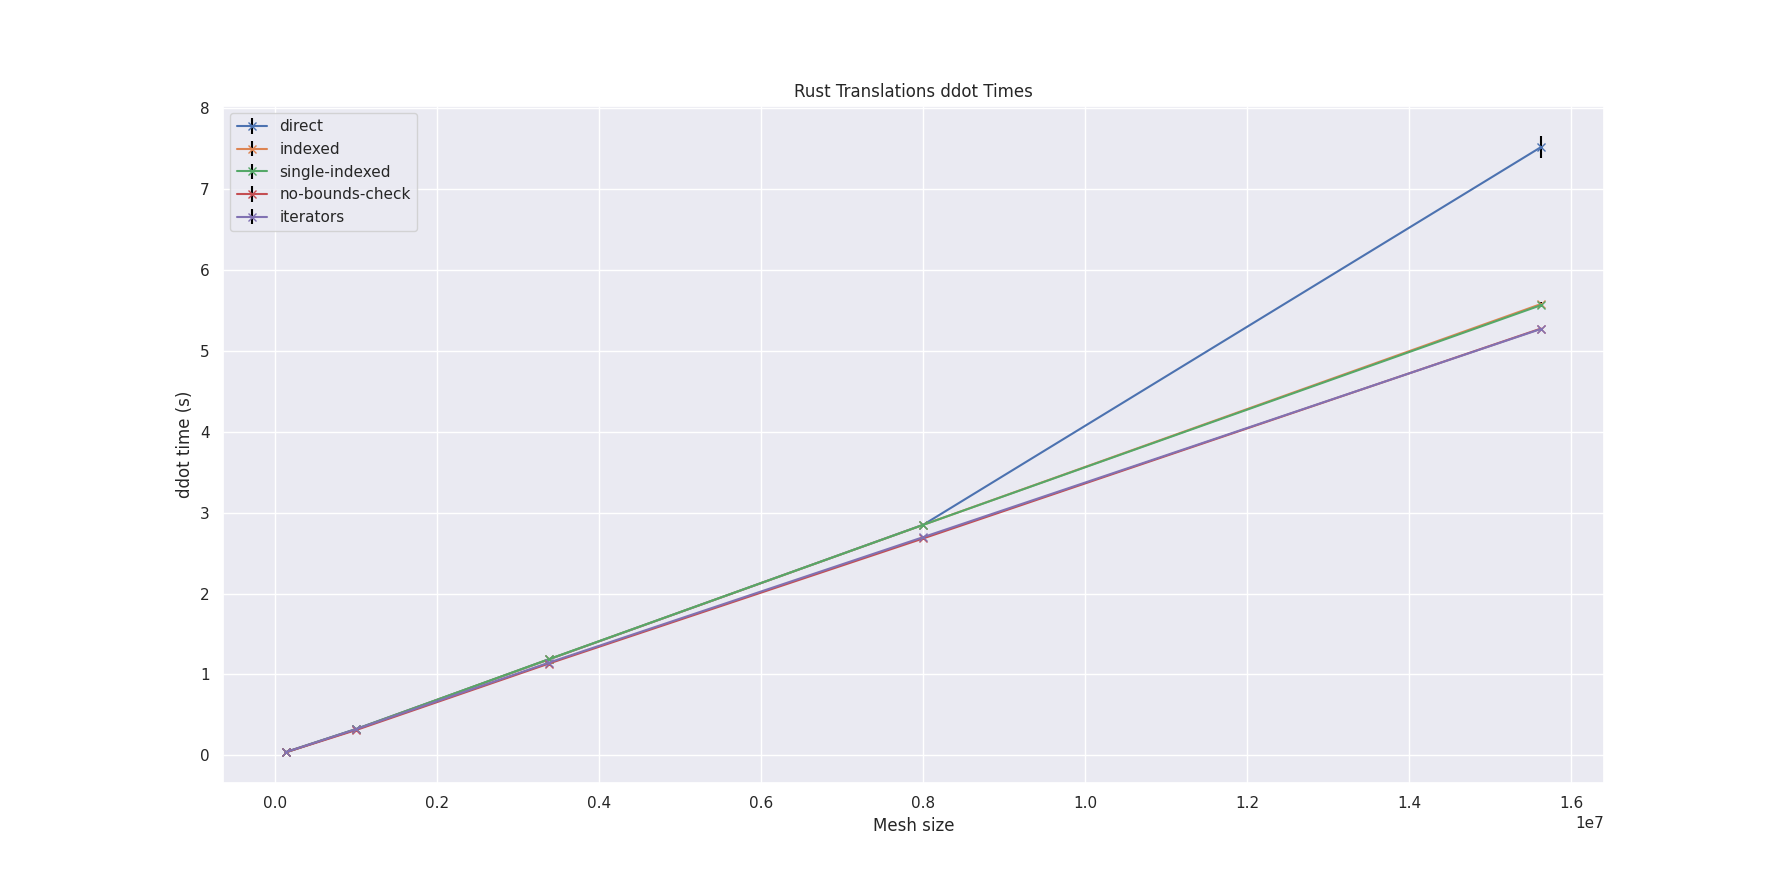
\includegraphics[width=\textwidth]{images/3_translation/performance/translations_ddot_line.png}
%     \caption{A diagram showing the wall time taken for the ddot kernel only of each translation, as the overall mesh size is varied.}
%     \label{fig:translations_ddot_line}
% \end{figure}

% \begin{figure}[H]
%     \centering
%     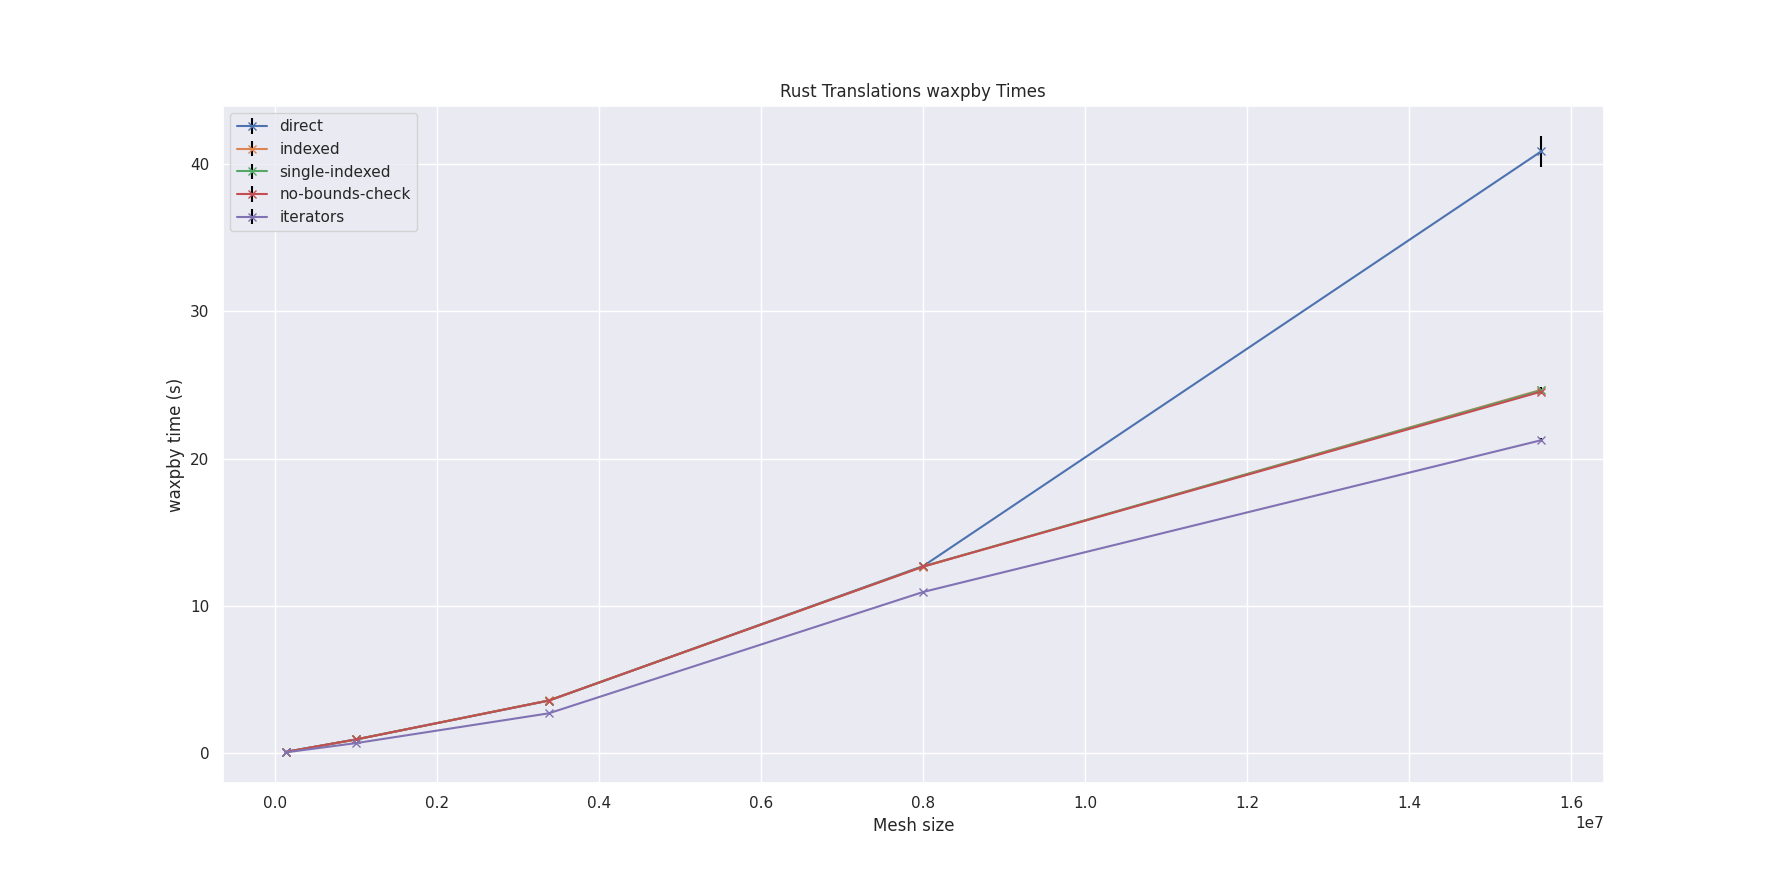
\includegraphics[width=\textwidth]{images/3_translation/performance/translations_waxpby_line.png}
%     \caption{A diagram showing the wall time taken for the waxpby kernel only of each translation, as the overall mesh size is varied.}
%     \label{fig:translations_waxpby_line}
% \end{figure}

% % TODO: Consider moving these summary charts to the performance analysis section?
% In addition to characterising how different translations affect performance, we can also get a preliminary understanding of the efficacy of different parallelism techniques in Rust. Figure \ref{fig:translation_parallelism_rust} shows the relative performance as characterised by the scaling of total wall time for serial, multi-threaded, MPI, and hybrid translations of the HPCCG mini-app.

% \begin{figure}[H]
%     \centering
%     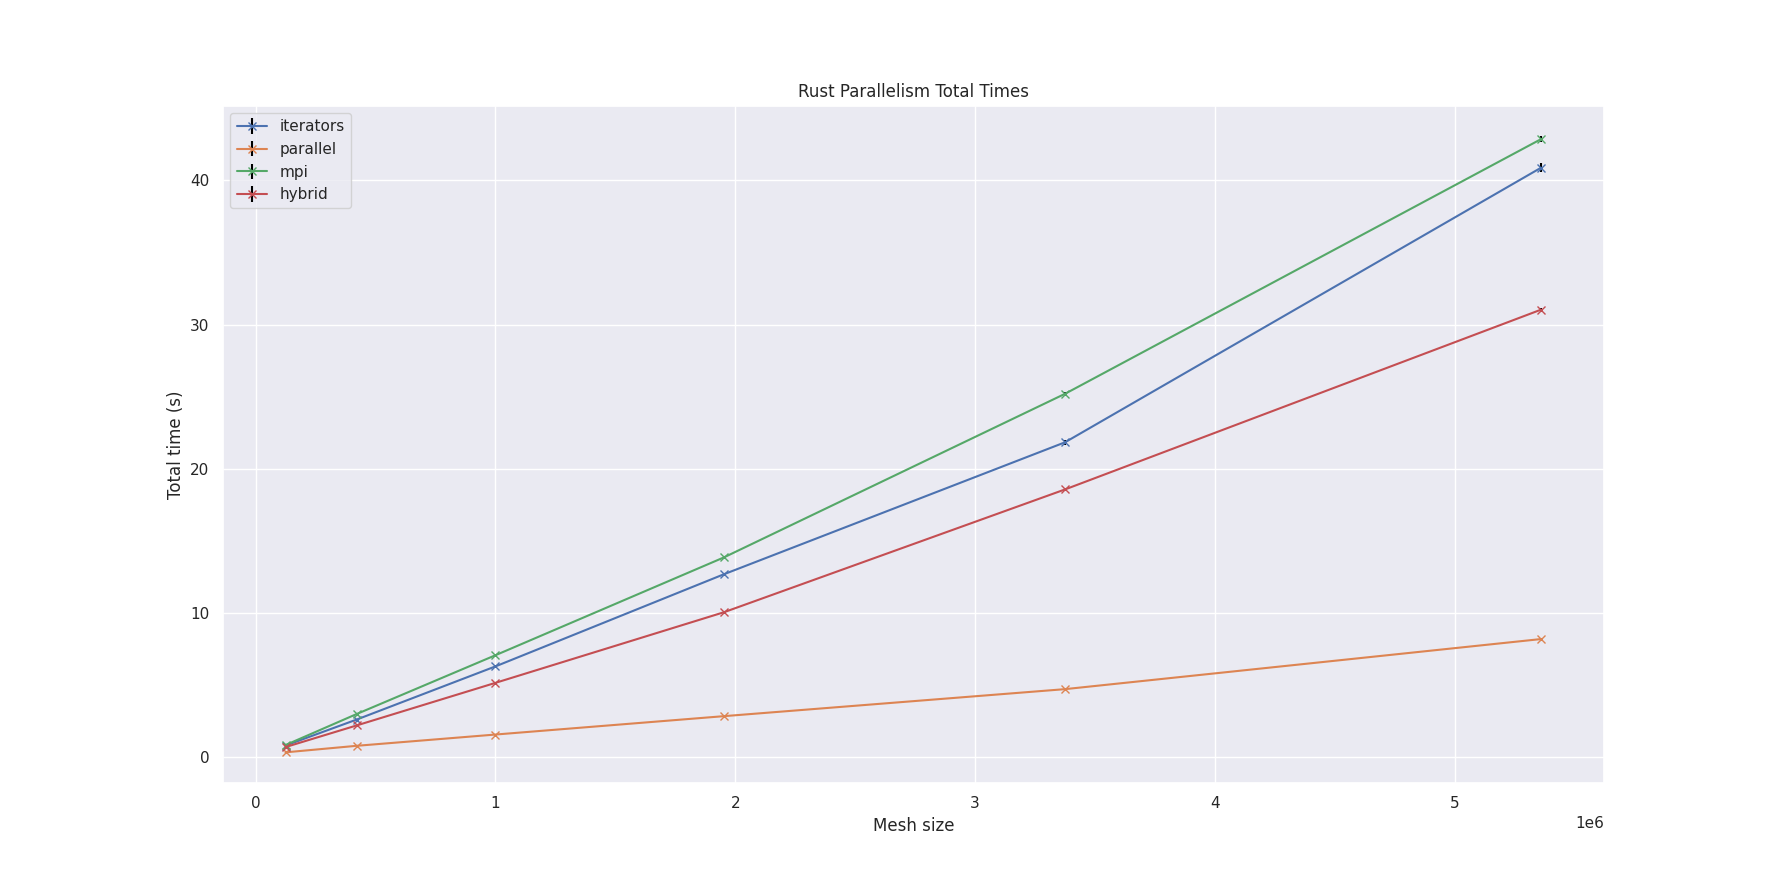
\includegraphics[width=\textwidth]{images/3_translation/performance/translation_parallelism_rust.png}
%     \caption{A diagram showing the total wall time taken for Rust implementations of parallelism approaches, as the overall mesh size is varied.}
%     \label{fig:translation_parallelism_rust}
% \end{figure}

% Here we can see that multi-threading is by far the most performant for small workloads on a single computer node. However, message passing approaches provide the capability to scale processing to clustered compute resources beyond the shared memory architecture of a single machine, and can be used in combination with multi-threaded approaches.

% Figure \ref{fig:translation_parallelism_cpp} shows the same experiments run over the parallelism methodologies of the C++ codebase. From this we can see that very similar trends hold, with the only difference being the Rust MPI implementation is slightly slower. A likely cause for this is the overhead as a result of the Rust bindings into the C++ implementation of the MPI specification.

% \begin{figure}[H]
%     \centering
%     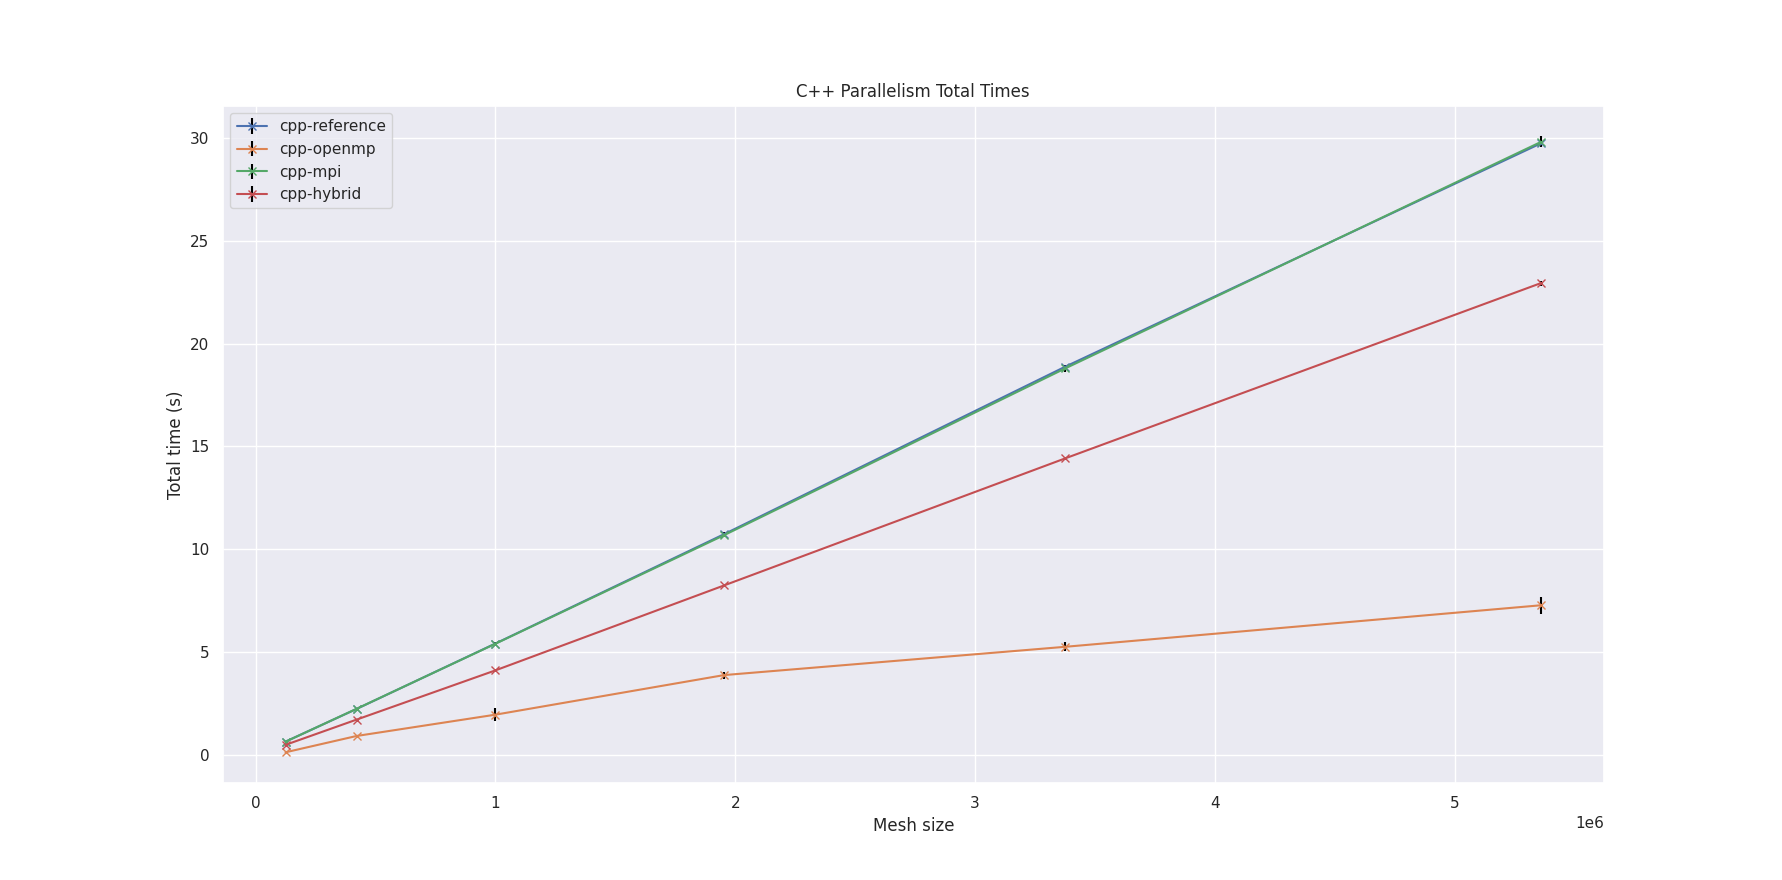
\includegraphics[width=\textwidth]{images/3_translation/performance/translation_parallelism_cpp.png}
%     \caption{A diagram showing the total wall time taken for C++ implementations of parallelism approaches, as the overall mesh size is varied.}
%     \label{fig:translation_parallelism_cpp}
% \end{figure}

In summary, the translation effort resulted in a performant implementation of the HPCCG mini-app in Rust, supporting both shared-memory parallelism through \texttt{rayon}, along with the stretch goal of distributed memory parallelism through the Rust MPI bindings. In addition to this, the Rust implementations of parallelism approaches shared similar performance characteristics to their C++ counterparts. This demonstrates that it is possible to use Rust for High-Performance Applications, for which HPCCG is representative workload. However, there are still aspects of Rust which add difficulty to this process, such as the state of the documentation of the Rust bindings to MPI -- but this is likely to improve in the future as Rust and its ecosystem matures.


\section{Equivalence checking}
\label{sec:equivalence-checking}

Equivalence checking is necessary to make performance comparisons between programs fair. In order to draw conclusions about the performance of the Rust translation of HPCCG, there must be strong confidence that it provides the same functionality as the C++ version. Taking this to its logical extremes, a Rust program which immediately terminates will have a much lower total runtime than the C++ implementation of HPPCG, but it clearly would not be a fair comparison of Rust and C++.
% However, the usefulness of equivalence checking is not only for ensuring performance comparisons are fair. Any translation effort from existing C++ code to Rust ...
To provide this confidence, four approaches for equivalence checking translated codebases were investigated: end-to-end testing, formal methods, comparison of intermediate representations, and unit testing.

\subsection{End-to-end testing}
\label{ssec:equivalence-end-to-end}

The simplest form of equivalence checking is end-to-end testing. This refers to running programs with the same input data, and asserting that they yield the same outputs. A key benefit of this approach is its simplicity -- no extra instrumentation or programming effort is required, only running the program as it would be run in a production application. As a result of this, it is difficult to implement incorrectly, so can be used as a ``sanity check'' to identify issues in other more complex testing apparatus.

However, end-to-end testing has a number of drawbacks, which primarily stem from its weak guarantees of test coverage. For example, a single set of input data may not fully exercise the control flow of the program, so cannot identify non-equivalent code in these areas which are not executed. The impact of this depends on the structure of the program, as single inputs to programs with many different conditional branches will only exercise a small proportion of the program, but for programs with only a single path of execution would exercise all of them.

During the development of the Rust translation of HPCCG, end-to-end testing was used to quickly test that minor changes to implementation did not obviously break program equivalence. This was broadly effective, as HPCCG has few conditional branches, so end-to-end testing provides high code coverage. This was then complemented by applying further verification techniques at less frequent intervals.

In summary, end-to-end testing can be effectively leveraged as part of an equivalence checking methodologies, with its simplicity encouraging developers to regularly check for obvious signs of broken equivalence. However, it is does not provide strong guarantees of equivalence, especially for highly branching code, so is best used in combination with other verification techniques.

\subsection{Formal methods}
\label{ssec:equivalence-formal-methods}

Another approach to equivalence checking is formal methods. R. Butler defines such approaches as ``mathematically rigorous techniques and tools for the specification, design and verification of software and hardware systems'' \cite{LangleyFormalMethods}. These approaches are most commonly applied to critical components in hardware design, where a single error could break a silicon tape-out, each of which cost in the order of millions of pounds.

One of the earliest applications of formal methods to proving program correctness was Hoare logic \cite{hoareAxiomaticBasisComputer1969}. Hoare logic is a sequence of triples representing atomic steps in programming execution and their pre and post conditions, along with inference rules to express constructs in imperative programs. By the application inference rules, theorems about properties of programs can be proven. Such approaches are desirable as they provide strong guarantees of correctness, but unfortunately they are exceedingly difficult to apply to non-trivial programs.

Furthermore, traditional formal methods are not well suited to checking equivalence between programs in different languages. This is because proofs exist within the formal system, but rely on a process to convert programs into these systems. The difference in program semantics between languages means that building a conversion algorithm which is consistent across two languages is almost impossible.

\subsection{Intermediate representation comparison}
\label{ssec:equivalence-ir-comparison}

A further possible approach to equivalence checking is the comparison of assembly or intermediate representation emitted by the compiler. LLVM is a modular framework for compilation originally presented by Latner and Adve in 2004 \cite{lattner2004llvm}, which has since gained popularity, in part due to its ability to generate optimised code irrespective of language. First, language-specific front-end converts the semantics of the program into LLVM IR. Then, LLVM's language independent middle-end applies transformations passes to the optimise the LLVM IR, which is structured to be amenable to this process. Finally, LLVM's hardware-specific back-end converts LLVM IR into appropriate machine code.

Since both C++ and Rust have compilers which use the LLVM framework, \texttt{clang} and \texttt{rustc} respectively, the HPCCG codebases can both converted into LLVM IR. If the programs are equivalent, these generated intermediate representations express the same functionality. As such, the intermediate representation may be similar. This process was attempted for a simple kernel, calculating the vector dot product, using the commands shown in Listing \ref{listing:llvm-ir-generation}, which both generate \texttt{ddot.ll} files containing the LLVM IR.

\begin{code}
    %TC:ignore
    \begin{minted}{bash}
    rustc --emit=llvm-ir --crate-type=lib ddot.rs
    clang++ -cc1 ddot.cpp -emit-llvm
    \end{minted}
    %TC:endignore
    \caption{The \texttt{rustc} and \texttt{clang++} invocations to generated LLVM IR for the vector dot product kernel in HPCCG.}
    \label{listing:llvm-ir-generation}
\end{code}

Unfortunately, the program models of Rust and C++ appear to generate quite different intermediate representations, even for simple kernels. For example, Rust's approach to bounded iteration leverages iterators, which results in quite different intermediate representation to C++'s loops which directly increment a mutable variable.

This methodology for equivalence checking may be possible, but would be an involved process to develop tooling to support this. As such, it was decided that comparison of intermediate representation was out of scope for this project, allowing the author to focus on more attainable tooling development, such as the HPC MultiBench tool.

\subsection{Unit testing}
\label{ssec:equivalence-unit-testing}

Unit testing refers to testing small components of the overall codebase, such as individual functions, to ensure they have the desired functionality. Since these tests are small in size typically many tests are written, then they are all executed together automatically \cite{archiveddocsTestEarlyOften2012}. A common design pattern for unit tests is the ``Arrange-Act-Assert'', where the data to drive the unit is set up, the unit is executed, and finally the output of the unit is checked. The metric of code coverage is often used to assess banks of unit tests, and refers to the proportion of lines in the codebase which are executed across all the tests.

As the software development industry has matured over the past decades, development methodologies have been created to formalise good practices during development. Test-Driven Development refers to a three stage cycle for software development, as shown in Figure \ref{fig:excalidraw_tdd}. First, a failing unit test is written exercise the intended behaviour. Next, ``just enough'' code is written to make the failing unit test pass. Finally, the code is refactored and the cycle starts again for the next feature \cite{beckTestDrivenDevelopment2022}.

\begin{figure}[H]
    \centering
    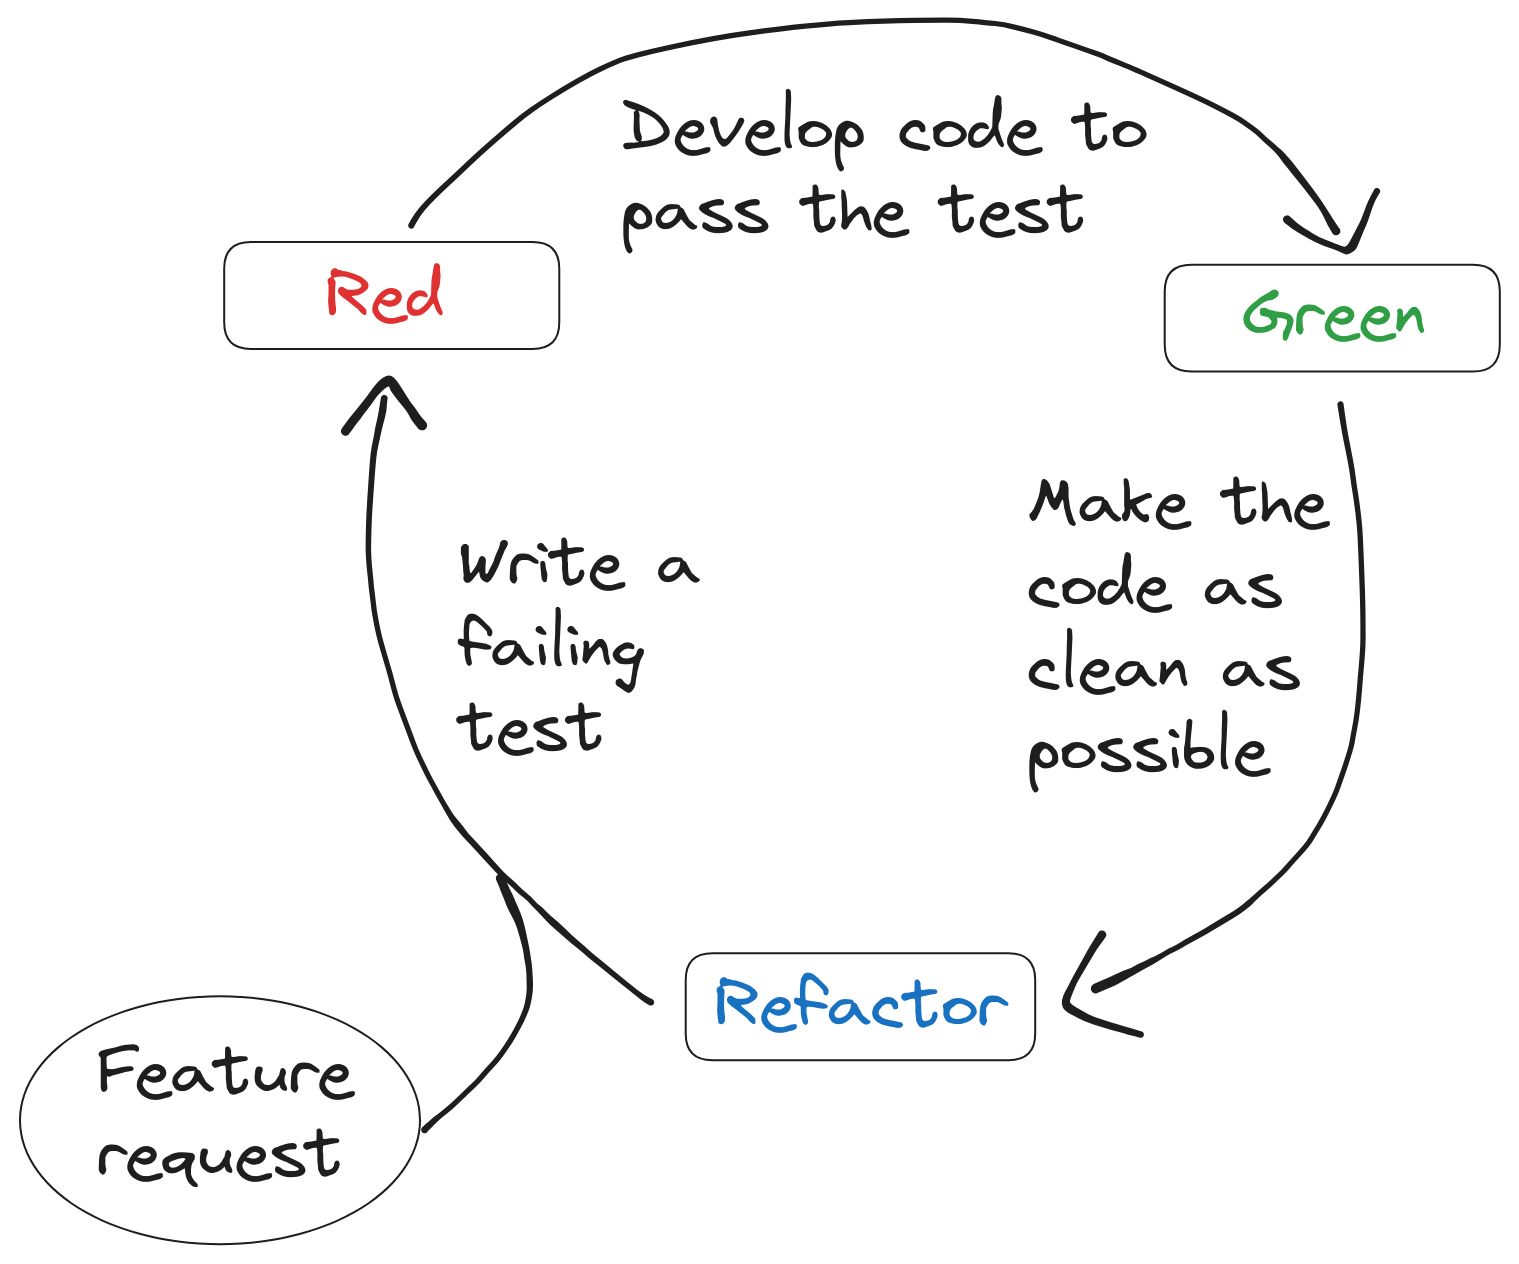
\includegraphics[width=0.5\textwidth]{images/3_translation/excalidraw_tdd.png}
    \caption{A diagram to showing the stages of the Test-Driven Development methodology.}
    \label{fig:excalidraw_tdd}
\end{figure}

The key and novel insight of applying unit tests to equivalence checking is that \textit{shared passing unit tests on both the original and translated implementations gives strong guarantees of equivalence}. More specifically, if two unit tests in different languages have semantically equivalent ``Arrange'' and ``Assert'' phases, and ``Act'' phases binding to their implementation of the unit under test, then passing unit tests guarantee that the tested functionality is shared by both languages. If the test bank from the original language has high code coverage, or the functionality is developed using Test-Driven Development, then the entire relevant functionality of the codebase can be guaranteed to be equal.

% Beyond this, Test-Driven Development can be leveraged during the translation process without the key complaint of developers -- the time spent writing tests. The cycle shown in Figure \ref{fig:excalidraw_tdd} can be tightened to two phases: writing ``just enough'' code to pass a single test, then refactoring it and repeating till all functionality is captured.

The original C++ version of HPCCG does not provide unit tests. As such, a set of unit tests for the C++ version had to be written before they could be leveraged for equivalence checking. The C++ Catch2 \cite{CatchorgCatch22024} framework was used to implement these tests, for example for the vector dot product kernel shown in Listing \ref{listing:cpp-ddot-unit-test}, as it is lightweight and simple to install.

\begin{code}
    %TC:ignore
    \begin{minted}{c++}
        #include <catch2/catch_test_macros.hpp>
        #include "../src/ddot.hpp"
        
        TEST_CASE("Test dot product implementation") {
            int width = 3;
            double lhs[] = {1.0, 2.0, 3.0};
            double rhs[] = {3.0, 2.0, 1.0};
            double result;
            double time_allreduce = 0.0;
            SECTION("Test differing lhs and rhs") {
                ddot(width, lhs, rhs, &result, time_allreduce);
                REQUIRE(result == 10.0);
            }
            SECTION("Test same lhs and rhs") {
                ddot(width, lhs, lhs, &result, time_allreduce);
                REQUIRE(result == 14.0);
            }
        }
    \end{minted}
    %TC:endignore
    \caption{A C++ implementation of unit tests for the vector dot product kernel, using the Catch2 test framework.}
    \label{listing:cpp-ddot-unit-test}
\end{code}

Translated code often has a similar internal structure to the reference implementation, for example internal methods which have the same functionality and provide the same functionality. As a result of this, having written the bank of C++ unit tests, they could be translated to Rust alongside the functions they drive, as the structure remains similar. For example, Listing \ref{listing:rust-ddot-unit-test} shows a Rust translation of the C++ unit test shown in Listing \ref{listing:cpp-ddot-unit-test}, having the same arrange and assert phases, but with the act phase driving the Rust and C++ functions respectively.

\begin{code}[H]
    %TC:ignore
    \begin{minted}{rust}
        #[test]
        fn test_ddot() {
            let width = 3;
            let lhs = vec![1.0, 2.0, 3.0];
            let rhs = vec![3.0, 2.0, 1.0];
            let result = ddot(width, &lhs, &rhs);
            assert_eq!(result, 10.0);
            let result = ddot(width, &lhs, &lhs);
            assert_eq!(result, 14.0);
        }
    \end{minted}
    %TC:endignore
    \caption{A Rust implementation of unit tests for the vector dot product kernel.}
    \label{listing:rust-ddot-unit-test}
\end{code}

By driving code units which should be equivalent across translations with the same arrangement of data, then asserting they produce the same results, strong guarantees of unit equivalence can be achieved. In addition to this, using the \texttt{tarpaulin} crate \cite{xd009642Xd009642Tarpaulin2024} to measure code coverage of the Rust unit tests, we can see that they provide full coverage over all functions excluding timing code and the main function which dispatches the solver. 

This combination of full code coverage and guarantees of equivalence for the tested properties of each unit gives strong confidence in the overall equivalence of the program. However, the process of translating these tests is manual and can be tedious for large banks of tests. As a result of this, it can be susceptible to human error -- which weakens the confidence in the equivalence checking process.

\subsubsection{Automating the novel approach}
\label{sssec:equivalence-polyglotest}

To strengthen the confidence and reduce the tedium of this process, we propose an automated methodology to facilitate writing Rust translations in this way. Using the \texttt{autocxx} crate, a foreign function interface between the two languages can be generated. Hence, the unit tests of one can invoke the code units of both itself and the other, as shown in Listing \ref{listing:rust-autocxx-bindings}.

\begin{code}
    %TC:ignore
    \begin{minted}{rust}
        include_cpp! {
            #include "ddot.hpp"
            safety!(unsafe_ffi)
            generate!("ddot")
        }
    \end{minted}
    %TC:endignore
    \caption{Using an \texttt{autocxx} macro in Rust to generate foreign function interface bindings to the C++ implementation of the dot product kernel.}
    \label{listing:rust-autocxx-bindings}
\end{code}

Having created this binding, Listing \ref{listing:rust-autocxx-unit-test} shows how it can be leveraged to multiplex between the driving the Rust and C++ codebases, with shared ``Arrange'' and ``Assert'' phases.

\begin{code}
    %TC:ignore
    \begin{minted}{rust}
        #[test]
        fn test_ddot() {
            let width = 3;
            let lhs = vec![1.0, 2.0, 3.0];
            let rhs = vec![3.0, 2.0, 1.0];
            let result = if TEST_RUST {
                ddot(width, &lhs, &rhs)
            } else {
                let mut result = 0.0;
                let mut tmp = 0.0;
                unsafe {
                    ffi_ddot(
                        c_int(width as i32),
                        lhs.as_ptr(),
                        rhs.as_ptr(),
                        &mut result,
                        Pin::new(&mut tmp),
                    );
                }
                result
            };
            assert_eq!(result, 10.0);
        }
    \end{minted}
    %TC:endignore
    \caption{.}
    \label{listing:rust-autocxx-unit-test}
\end{code}

The combination of these two listings constitute a proof-of-concept for a translation development methodology which leverages automated testing techniques to provide strong guarantees of program equivalence between languages with very different semantics. A developer would write unit tests in Rust to fully exercise the C++ code with the \mintinline{rust}{TEST_RUST} flag unset. Then, when the unit tests has been completed, the \mintinline{rust}{TEST_RUST} flag can be set. The developer now has a full bank of unit tests, which they can select from and implement functionality for until an equivalent program is written, drawing inspiration from the Test-Driven Development methodology.

% % TODO: How important is this section?
% \section{Lessons learned and proposed workflow} 
% \label{sec:translation-workflow}
% % Translation stuff
% % Equivalence checking stuff


\section{Developer productivity}
\label{sec:developer-productivity}

As discussed in the literature review, Diehl et al. use a COCOMO model to estimate the developer effort required across languages to implement the same functionality \cite{diehlBenchmarkingParallel1D2023}. They conclude that Rust requires slightly less developer effort by comparing the quantitative results of this model.

The \texttt{scc} tool counts lines of code, and uses a COCOMO model to quantitatively estimate developer effort. Table \ref{tab:scc-language-comparison} shows the results of running this tool on the source directories of the Rust and C++ implementations, both leveraging shared and distributed memory parallelism. For all metrics shown in the table, smaller is better.

% TODO: Update based on stripped codebases using unifdef tool?
\begin{table}[H]
    \centering
    \caption{The results of running the \texttt{scc} on the C++ and Rust implementations of HPCCG, quantitatively assessing developer productivity.}
    \label{tab:scc-language-comparison}
    \begin{tabular}{|l||l|l|l|}
    \hline
    \textbf{Metric}             & \textbf{Rust} & \textbf{C++} & \textbf{Rust scale factor} \\ \hline\hline
    Lines of code               & 999           & 1595         & 62.6\%                     \\ \hline
    Estimated complexity        & 116           & 224          & 51.8\%                     \\ \hline
    Estimated schedule (months) & 3.49          & 4.20         & 83.1\%                     \\ \hline
    Estimated cost (\$)         & 26986         & 44105        & 61.2\%                     \\ \hline
    \end{tabular}
\end{table}


% TODO: Decide whether this is funny/appropriate/too close to the bone...
% Under the crushing weight of capitalism, developer productivity can be most effectively assessed by the generation of shareholder value -- that is to say estimates of development cost for a fixed set of functionality. By the quantitative estimate of development cost shown in Table \ref{tab:scc-language-comparison}, Rust can be assessed as $1.5 \times$ more productive than C++. This contrasts Diehl et al.'s results of a very small impact in developer effort. Two possible reasons for this discrepancy is that the HPCCG is approximately five times larger in lines of code, and Diehl et al. do not consider MPI, for which the Rust bindings provide a terse API in comparison with the more verbose C++ specification implementation.
Developer productivity can be assessed as the generation of value for stakeholders -- that is to say estimates of development cost for a fixed set of functionality. By the quantitative estimate of development cost shown in Table \ref{tab:scc-language-comparison}, Rust can be assessed as $1.5 \times$ more productive than C++.

This contrasts Diehl et al.'s results of a very small impact in developer effort. Two possible reasons for this discrepancy is that the HPCCG is approximately five times larger in lines of code, and Diehl et al. do not consider MPI, for which the Rust bindings provide a terse API in comparison with the more verbose C++ specification implementation.

Beyond estimating costs by counting lines of code and applying complexity metrics, there are other tangible impacts on developer productivity provided by the Rust language. As discussed in \Cref{ch:background}, one example of this is Rust's guarantees of memory and concurrency safety, which significantly reduces the time spent debugging flaky bugs as such errors are moved from runtime to compile time.

A further example is Rust's robust toolchain, with \texttt{cargo} providing built tooling, package management, auto-formatting, and linting, all in a single convenient command. During the development process, a significant amount of time was spent migrating the C++ implementation build tooling from a Makefile to CMake in order to use the Kokkos performance portability package, which would take only a single command using the Rust toolchain.
